%base packages 
\documentclass[11pt]{article}
\usepackage[margin=1in]{geometry}
\usepackage{caption,multirow,etoolbox,color,enumerate,amsmath,dsfont,lscape,tocloft,booktabs,draftwatermark,array,tabularx,graphicx,pdflscape,subcaption}
\usepackage{setspace}
\setlength{\parskip}{0em}
\usepackage[bottom, flushmargin]{footmisc}
\usepackage[T1]{fontenc}
\usepackage[utf8]{inputenc}
\usepackage{lmodern}
\usepackage[english]{babel}
\usepackage[autostyle]{csquotes}
\makeatletter
\makeatother
\usepackage{float}
\SetWatermarkText{}\SetWatermarkLightness{0.85} \SetWatermarkScale{4}
\usepackage{appendix}
\usepackage{authblk}
\usepackage[format=hang,justification=raggedright,singlelinecheck=0,labelsep=period]{caption}
%[format=hang,justification=raggedright,singlelinecheck=0,labelsep=period]
%\usepackage[numbers,sort&compress]{natbib} %Use this set-up for numbered reference lists
\usepackage[authoryear]{natbib} %Use this set-up if you want an un-numbered reference list
%\usepackage{hypernat}

\usepackage[hyperfootnotes=false]{hyperref}
%\usepackage[dvipdfmx,hyperfootnotes=false]{hyperref}
%\usepackage[dvips,hyperfootnotes=false]{hyperref}
\hypersetup{colorlinks=true,linkcolor=blue,anchorcolor=blue,citecolor=blue,filecolor=blue,urlcolor=blue,bookmarksnumbered=true,pdfview=FitB} %
% % %DO NOT PLACE ANY PACKAGES AFTER THE HYPERREF SET UP
\usepackage{titling}

%-----------------------------------------------------------------------%
\begin{document}
\bibliographystyle{mla-good}


\title{Collective Action, Communication and the Coordination Challenge: An Analysis of Smallholder Livestock Cooperatives in Nepal \vspace{1cm}}

\author{Scott M. Miller}
\date{}

\sloppy
\maketitle

\begin{center}
    \large{Dissertation Proposal}
\end{center}

\vspace{2cm}

Committee Chair: Dr. Conner Mullally \\

Committee Members: Dr. Travis McArthur \\

\hspace{1.45in} Dr. Spiro Stefanou \\

\hspace{1.45in} Dr. Renata Serra\footnote{External committee member} \\




%------------------------------------------%
%\begin{abstract}
%
%\end{abstract}
%------------------------------------------%

\pagenumbering{gobble}
\clearpage
\renewcommand{\cftsecleader}{\cftdotfill{\cftdotsep}}

\tableofcontents
\clearpage

\doublespacing
\thispagestyle{plain}
\pagenumbering{arabic}
\setcounter{page}{1}

%-----------------------------------------------------------------------%
\section{Introduction} \label{sec:intro}
% Hook
%Many of the world's poorest households live in rural areas and 
Two-thirds of the world's poorest households live in rural areas and depend on agriculture for their livelihoods \citep{fugile-et.al.19}. Tackling poverty, hunger and malnutrition require drastically increasing the production and commercialization of smallholder agricultural producers \citep{fisher-qaim12,worldbank08}. Although productivity growth in agriculture has the largest impact of any sector on reducing poverty \citep{fugile-et.al.19}, rural markets in developing countries are often rife with constraints that limit the ability of smallholders to sell in formal markets \citep{ashby-et.al.09,kristjanson-et.al.14}. These constraints include poor infrastructure, weak communication channels and long distances between market actors that lead to high transaction costs, weak bargaining power and information asymmetry \citep{aker10,barrett.08,key.et.al.00,staal-et.al.97}. 

In the face of severe market constraints, agricultural cooperatives often arise in an effort to increase bargaining power, decrease transaction costs, and help achieve scale economies in marketing \citep{markelova-et.al.09,rondot-collion01,staal-et.al.97,worldbank03}. By exploiting the potential of collective action, cooperatives provide the opportunity for smallholders to access markets that may otherwise be inaccessible, pool resources to overcome financial constraints, increase communication flows and collectively negotiate with buyers to receive better prices \citep{poole-defrece10}. However, rather than eliminating the source of market constraints, the burdens are shifted to the cooperatives themselves. The effectiveness of cooperatives in raising smallholder market engagement will depend on how well cooperatives manage the challenge of internally coordinating sales among a large group of individual market actors. Evidence suggests that some farmer organizations are able to successfully overcome this challenge, generating large and inclusive benefits for their members \citep{narrod-et.al.09,tadesse-bahiigwa15,wollni-zeller07}. Others largely fail in this effort, resulting in a high presence of side-selling, heterogeneous benefits, or dissolving participation among their members \citep{aflagah-et.al.19,bernard-spielman09, casaburi-macchiavello15}. 

Which factors influence the success and failure of agricultural cooperatives and how can researchers, policymakers and NGOs promote thriving producer organizations? I answer these questions by i) decomposing the cooperative performance gap between the most and least inclusive cooperatives, ii) analyzing the role that comparative advantage plays in cooperative participation decisions, and iii) assessing the impacts of a smartphone application that is designed to improve cooperative performance by relaxing the constraints associated with arranging sales. My population of interest are smallholder goat producers in rural Nepal, all of whom are women and members of agricultural cooperatives. All three of my essays will draw on a comprehensive panel dataset that consists of over 2,800 households across 109 cooperatives in Nepal.

In my first essay, I propose to investigate the tradeoff between inclusive membership and market performance performance in agricultural cooperatives. An important issue highlighted in the cooperative literature is the equity-efficiency tradeoff, where producer organizations struggle to balance social inclusion with market competitiveness \citep{bernard-spielman09,worldbank08}. However, it is not clear whether the inverse relationship between inclusiveness and performance is driven by observable differences in cooperative characteristics or unobservable differences in their ability to translate those characteristics into performance. In order to further examine this relationship, I use the \citet{oaxaca73}-\citet{blinder73} decomposition to estimate i) whether there is a significant performance gap between the most and least inclusive cooperatives, and ii) whether this gap is best explained by observable differences between cooperatives or differences in their ability to achieve market performance. 

In my second essay, I propose to estimate the distribution of net returns to selling through the cooperative in order to analyze the role that comparative advantage plays in cooperative participation. In my data, I observe extensive side-selling, despite evidence that those who sell through the cooperative earn a higher price and sell more output, on average. In order to disentangle this puzzle, I will estimate a correlated random coefficient model, following \citet{suri11}, where the adoption choice is to sell through the cooperative rather than to a local trader. This estimation will allow me to determine whether there are significant net returns to cooperative sales, if these returns heterogeneous and if so, whether or not this heterogeneity explains the side-selling decision. By understanding the distribution of returns to adoption, I will be able to discuss the role that comparative and absolute advantage play in cooperative participation decisions. 

In my third essay, I propose to evaluate the effects of a smartphone-based, information-sharing app for livestock producers known as the ``Virtual Collection Center'' (VCC). The VCC allows rank-and-file cooperative members to regularly update leadership on available goat inventory. Cooperative leaders use inventory information to negotiate bulk sales with traders, and then invite cooperative members to sales events through the app. By lowering barriers to communication in an environment characterized by rugged terrain and long travel times between population centers, the VCC has the potential to encourage market participation by cooperative members, thereby raising incomes. This intervention will be evaluated through a cluster-randomized control trial, with treatment randomly assigned at the cooperative level. 

%-----------------------------------------------------------------------%
\newpage
\section{Background \& Data} \label{sec:background}

In Nepal, where 68 percent of the population depends on agriculture for their livelihood \citep{ILO16}, goats are a common source of income and nutrition. This is particularly true in rural areas, where nearly every household owns a least a few goats for production and/or consumption \citep{upreti09}. In recent years, urbanization and rising incomes have lead to a higher demand for goat meat, but a poorly functioning value chain has left smallholder producers, most of whom are women, unable to benefit \citep{ashby-et.al.09,choudhary-et.al.11,gurung-et.al.15}. Smallholders face high transaction costs, weak bargaining power and a lack of communication infrastructure that limit their ability to access and gain from formal output markets \citep{ashby-et.al.09,kristjanson-et.al.14}. As a result, domestic production has been unable to keep up with rising demand, leading to higher imports from India and Tibet \citep{HI-N12}.

Many agricultural policy and rural development plans in Nepal have promoted agricultural cooperatives as a means of supporting smallholder producers \citep{ADS15}. Non-governmental organizations, including Heifer Project International in Nepal (HPIN), have made recent efforts to strengthen the goat value chain by organizing producer cooperatives. HPIN’s programs give women livestock and extensive training. Beneficiaries are then organized into self-help groups (SHGs) of around 20-30 female members. Once SHGs in a given area are sufficiently organized, they are combined into larger producer cooperatives \citep{janzen-et.al.18}.

% This follows closely from the VCC Pre-Analysis Plan. In the full dissertation, I will cite this accordingly if that paper moves forward
The majority of goats in Nepal are consumed after sale to a local collector who pools animals from smallholder producers \citep{HI-N12}. For goats that are marketed outside of their original communities, the commercial value chain links producers, local collectors and regional traders to consumers who are primarily located in urban markets \citep{HI-N12}. A collector looking to buy goats from smallholder producers who are not affiliated with a cooperative would likely have to conduct individual negotiations, sometimes making multiple visits per home \citep{HI-N12, staal-et.al.97}. After agreeing to terms with producers, the collector would still have to coordinate transportation. If the collector does not want to transport goats from each individual home, then he or she would have to arrange for producers to bring their animals to a collection point at a specific date and time. Bargaining with many small producers and managing logistics may inflate transaction costs and dissuade collectors from dealing with smallholders. In contrast, a collector purchasing through a cooperative need only negotiate with a single entity and can leave sales coordination to cooperative managers.

%-----------------------------------------------------------------------%
\subsection{Data} \label{sec:data}
The data used throughout this dissertation were originally collected as baseline and endline data for a randomized control trial, which is the subject of Section \ref{sec:E3} of this proposal. The sample frame of this dataset is a list of 109 cooperatives spread across four of five development regions in Nepal, specifically the East, Central, West and Mid-Western Development regions. All cooperatives operate in either the low-land Terai or mid-Hills. Figure \ref{map} shows the study area covered in the sample, which includes cooperatives from 24 districts across Nepal. The cooperatives included in the study were selected by HPIN and include all existing livestock marketing cooperatives the organization helped form prior to 2017.

\begin{figure}[!h]
    \caption{Study Area}
    \label{map}
    \noindent \centering 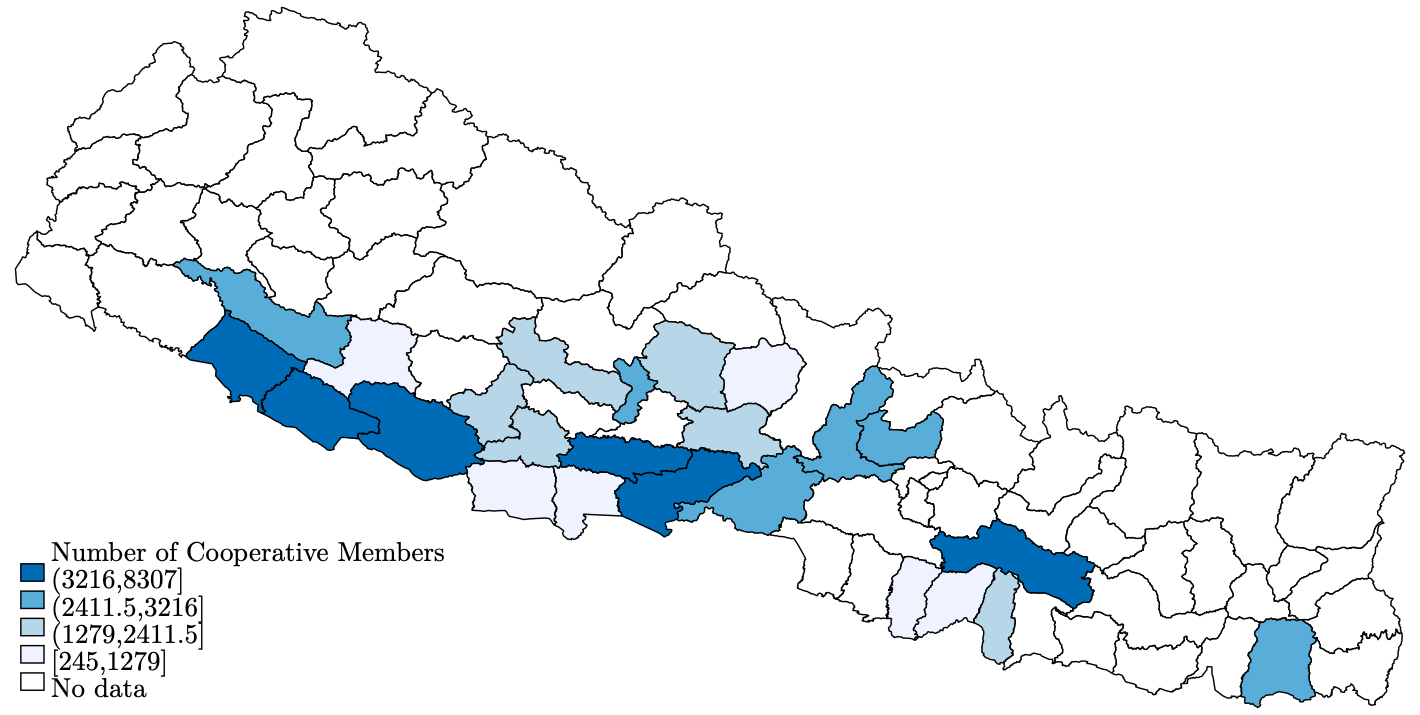
\includegraphics[width=.75\textwidth]{StudyMap.png}
\end{figure}

This dataset consists of two separate surveys - one with cooperative leaders and another with general members.  I refer to these surveys as the cooperative leader and household survey, respectively. The cooperative leader survey is comprised of interviews from three officers in each cooperative. To obtain a representative sample for the household survey, HPIN and cooperative leaders generated complete cooperative rosters. From these comprehensive lists, a random sample of 2,856 households across 109 cooperatives was drawn to participate in the household survey. The first round of data were collected from the sample in January 2018 using Android tablets and Open Data Kit. A second round of data will be collected in February 2020.

%\newpage
\singlespacing
% Summary Stats Table
\newcolumntype{Y}{>{\centering\arraybackslash}X}
\begin{table}[!h]
  \centering
  \caption{Summary Statistics (2018 Sample)}
  \label{table:summary}
  \scalebox{.8}{
  \begin{tabularx}{1.2\linewidth}{l*{7}{Y}}
\hline Cooperative-Level Variables & N & Mean & sd & Min & Max\\
\noalign{\smallskip}\hline \noalign{\smallskip}
Number of Members (count) & 107.00 & 568.64 & 375.77 & 11.00 & 2,600.00\\
Annual Revenue (USD) & 108.00 & 3,862.05 & 7,503.18 & 0.00 & 65,709.51\\
Annual Costs (USD) & 108.00 & 624.62 & 2,619.28 & 0.00 & 21,383.74\\
Annual Net revenue (USD) & 106.00 & 3,298.52 & 7,929.31 & -16,676.6 & 65,554.2\\
Annual Revenue per member (USD) & 108.00 & 7.26 & 10.34 & 0.00 & 63.53\\
Annual Net revenue per member (USD) & 105.00 & 6.44 & 10.94 & -29.78 & 63.53\\
Annual Goat revenue (USD) & 106.00 & 173.05 & 542.82 & 0.00 & 5,262.24\\
Planning time horizon (years) & 108.00 & 1.33 & 1.07 & 0.00 & 5.00\\
ICT assets (count) & 108.00 & 0.62 & 0.71 & 0.00 & 3.00\\
Non-ICT assets (count) \hspace{2.15in} & 108.00 & 2.85 & 2.36 & 0.00 & 15.00\\


  \end{tabularx}}
  \scalebox{.8}{
  \begin{tabularx}{1.2\linewidth}{l*{7}{Y}}
\hline Household-Level Variables & N & Mean & sd & Min & Max\\
\noalign{\smallskip}\hline \noalign{\smallskip}
Age of female cooperative member (years) & 2,856.00 & 42.35 & 11.58 & 20.00 & 83.00\\
Literacy of female cooperative member (0/1) & 2,856.00 & 0.79 & 0.36 & 0.00 & 1.00\\
Contacted about cooperative sales in last 6-months (0/1) & 2,856.00 & 0.35 & 0.48 & 0.00 & 1.00\\
Total number of goats owned (count) & 2,856.00 & 5.76 & 4.95 & 0.00 & 69.00\\
Household sold goats in the last 12-months (0/1) & 2,856.00 & 0.48 & 0.50 & 0.00 & 1.00\\
Household side-sold goats in the last 12-months (0/1) & 1,384.00 & 0.77 & 0.42 & 0.00 & 1.00\\
Annual number of goats sold (count) & 1,384.00 & 2.31 & 1.85 & 1.00 & 10.00\\
Annual number of cooperative goats sold (count) & 1,384.00 & 0.53 & 1.05 & 0.00 & 4.00\\
Annual revenue per goat (USD) & 1,384.00 & 85.07 & 37.15 & 0.00 & 178.20\\
Annual revenue per cooperative goat (USD) & 353.00 & 91.44 & 30.08 & 0.00 & 135.13\\
Annual net goat income (USD) & 1,384.00 & 148.41 & 159.81 & -284.13 & 725.67\\
\hline
\multicolumn{6}{@{}p{1.2\textwidth}}
{\textit{Notes}: At the household-level, several variables include missing values and are conditional the household selling goats. These variables include: household side-sells goats, total goats sold, cooperative goats sold, revenue per goat and net goat income. Revenue per cooperative goat sold is conditional on the household selling goats through the cooperative.}
  \end{tabularx}}
\end{table}
\doublespacing

Table (\ref{table:summary}) displays summary statistics from the 2018 sample of my data. The average cooperative in my sample has 569 members, and a revenue of over \$3,800 USD. On average, cooperatives operate with a net revenue of roughly \$3,300 USD. However, there is significant heterogeneity in this measure, as average net revenue ranges from below -\$16,600 to more than \$65,500 USD. The average cooperative owns fewer than one information and communication technology (ICT) asset, but owns nearly 3 non-ICT assets. The average cooperative member in my sample is 42 years old, roughly 80\% of whom are literate. While the average household owns more than 5 goats, only 48\% sold a goat in the year prior to data collection and only 35\% received sale information from their cooperative in the 6-months prior to data collection. This may in part explain the disparity between goat sales through and outside of the cooperative. On average, goat-selling households sold more than two goats and received a revenue of \$85.07 USD per goat. Meanwhile, among goat-selling households the average number of cooperative goats sold is 0.53 and the average revenue per cooperative goat sold is \$91.44.


%-----------------------------------------------------------------------%
\newpage
\singlespacing
\section{Investigating the Inclusive-Performance Tradeoff in Agricultural Cooperatives} \label{sec:E1}
\doublespacing


% --------------------------------------
\subsection{Motivation} \label{sec:E1_motivation}

% Hook / Question
Is there a tradeoff between inclusive membership and market performance in agricultural cooperatives? The answer to this question is critical for understanding the role that cooperatives play in agricultural development and poverty alleviation. 
% Antecedents
The relationship between equity and efficiency has been highlighted as an unresolved conflict in the cooperative literature \citep{worldbank08}. In fact, \citet{bernard-spielman09} suggest that cooperatives can achieve only two of the following three conditions i) inclusive membership, ii) participatory decision-making and iii) market performance. However, it is not clear whether the inverse relationship between inclusiveness and performance is driven by observable differences in cooperatives or unobservable differences in their ability to translate those characteristics into results. The issue of selection bias has not been sufficiently addressed in the relevant literature, potentially obscuring the relationship of interest. 

% Value Added
In this essay, I propose to use the \citet{oaxaca73}-\citet{blinder73} decomposition to further examine this relationship and address the issue of selection bias. I will separate the inclusive performance gap into the portion that is explained by differences in observable characteristics and the portion that is explained by the returns to those characteristics. Although decomposition methods typically do not provide causal estimates, this approach closely follows the program evaluation literature, where the `unexplained' portion of the gap (i.e. returns to characteristics) is analogous to a treatment effect \citep{fortin-et.al.11}. This approach estimates separate linear regressions for each group and uses the resulting parameters to understand the expected outcome that one group could obtain if their characteristics matched those of the other group. Therefore, this approach to  provides a useful framework for better understanding the relationship between inclusiveness and market performance. %CM: I think these last two sentences could be explained a bit better. 

% --------------------------------------
\subsection{Data} \label{sec:E1_data}

In this essay, I use the full dataset discussed in section (\ref{sec:data}). To separately analyze the cooperative performance gap in absolute and growth terms, I will use a pooled cross-section and first-difference panel structure of the data, respectively. 

%\newpage
\singlespacing
% Summary Stats Table
\newcolumntype{Y}{>{\centering\arraybackslash}X}
\begin{table}[H]
  \centering
  \caption{Summary Statistics (2018 Sample)}
  \label{table:E1_summary}
  \scalebox{.8}{
  \begin{tabularx}{1.2\linewidth}{l*{7}{Y}}
\hline Cooperative-Level Variables & N & Mean & sd & Min & Max\\
\noalign{\smallskip}\hline \noalign{\smallskip}
Cooperative has an initial membership fee (0/1) & 107.00 & 0.93 & 0.26 & 0.00 & 1.00\\
Size of initial membership fee (USD) & 108.00 & 2.22 & 3.86 & 0.00 & 35.64\\
Size of current management committee (count) & 107.00 & 10.46 & 1.78 & 7.00 & 15.00\\
Share of members the attending last general assembly (count) & 108.00 & 0.64 & 0.27 & 0.00 & 1.00\\
Cooperative organizes goat sales (0/1) & 108.00 & 0.86 & 0.35 & 0.00 & 1.00\\
Cooperative accepts savings deposits (0/1) & 108.00 & 0.97 & 0.17 & 0.00 & 1.00\\
Cooperative offers loans (0/1) & 108.00 & 0.91 & 0.29 & 0.00 & 1.00\\
Cooperative provides goat price information (0/1) & 108.00 & 0.87 & 0.34 & 0.00 & 1.00\\
Cooperative pays dividends to share owners (0/1) & 108.00 & 0.66 & 0.48 & 0.00 & 1.00\\

  \end{tabularx}}
  \scalebox{.8}{
  \begin{tabularx}{1.2\linewidth}{l*{7}{Y}}
\hline Household-Level Variables & N & Mean & sd & Min & Max\\
\noalign{\smallskip}\hline \noalign{\smallskip}
Length of membership (years) & 2,856.00 & 3.04 & 1.84 & 0.00 & 9.00\\
Number of self-help group meetings attended (count) & 2,856.00 & 5.43 & 1.80 & 0.00 & 15.00\\
Number of cooperative meetings attended (count) & 2,856.00 & 1.76 & 2.45 & 0.00 & 24.00\\
Round-trip travel time to cooperative meetings (minutes) & 2,856.00 & 91.58 & 103.41 & 0.00 & 420.00\\
Participates in annual general meeting (0/1) & 2,856.00 & 0.69 & 0.46 & 0.00 & 1.00\\
Voted in elections in last 2-years (0/1) & 2,856.00 & 0.09 & 0.29 & 0.00 & 1.00\\
Voted on policies in last 2-years (0/1) & 2,856.00 & 0.03 & 0.17 & 0.00 & 1.00\\
Value of dividend payments received (USD) & 2,856.00 & 0.66 & 4.53 & 0.00 & 148.50\\
Contacted about cooperative sales in last 6-months (0/1) & 2,856.00 & 0.35 & 0.48 & 0.00 & 1.00\\
Contacted about cooperative activities in last 6-months (0/1) \hspace{.1cm} & 2,856.00 & 0.38 & 0.49 & 0.00 & 1.00\\
\hline
\multicolumn{6}{@{}p{1\textwidth}}
{\textit{Notes}: }
  \end{tabularx}}
\end{table}
\doublespacing

Table (\ref{table:E1_summary}) provides summary statistics from the 2018 sample of my data. While 93\% of cooperatives have an initial membership fee, the average cooperative charges \$2.22 USD. At the last general assembly meeting prior to data collection, only 64\% of members were in attendance, on average. More than 85\% of cooperatives indicate that they coordinate goat sales with traders and 87\% provide goat price information to their members. Meanwhile, 97\% accept savings deposits from their members and 91\% offer loans, but only 66\% provide dividend payments to the cooperative's shareholders. At the household level, the average member has been a part of their cooperative for 3 years. On average, members have attended more than five self-help group meetings in the 6-months prior to data collection, and attended fewer than two cooperative meetings over this period. Members indicate a round-trip travel time to the cooperative of more than 90 minutes, on average. While nearly 70\% of members indicate that they participate in the cooperative's general meeting, fewer than 10\% have voted in cooperative elections and only 3\% have voted on cooperative policies. The average household indicated receiving \$0.66 USD in dividend payments over the 6-months prior to data collection. Roughly 35\% of members were contacted about cooperative organized livestock sales in the 6-months prior to data collection, and 38\% were contacted about non-sale related cooperative activities. 


% --------------------------------------
\subsection{Empirical Strategy} \label{sec:E1_emp}

% --------------------------------------
\subsubsection{Theoretical Framework} \label{sec:E1_theory}

The \citet{oaxaca73}-\citet{blinder73} decomposition allows me to separate the observed average outcomes between the most and least inclusive cooperatives into an explained and an unexplained component. For example, suppose that the relationship between the outcome for farmer $i$, $Y_i$, and a vector of the determinants of performance, $\mathbf{X}_i$, can be written as

\begin{equation} \label{eq:E1_1}
    Y_i = \beta \mathbf{X}_i + \varepsilon_i
\end{equation}  

%CM: Be clear what \beta is. 
Given that the most and least inclusive cooperatives likely differ in their ability to translate farmer potential into performance, I will allow for different values of $\beta$ for each group. Using the group-specific parameters, the difference between average outcomes for the most and least inclusive cooperatives is written as:

\begin{equation} \label{eq:E1_2}
        \overline{Y}_{h} - \overline{Y}_{\ell} =  \beta_{h}\overline{\mathbf{X}}_{h} - \beta_{\ell}\overline{\mathbf{X}}_{\ell}
\end{equation}  

Rearranging this equation by adding and subtracting $\beta_{\ell}\overline{X}_{h}$ on both sides gives:

\begin{subequations}
    \begin{align}
        \overline{Y}&_{h} - \overline{Y}_{\ell} \label{eq:E1_3a} \\
        &= \beta_{\ell}[\overline{\mathbf{X}}_{h} - \overline{\mathbf{X}}_{\ell}] \label{eq:E1_3b} \\
        &+ \overline{\mathbf{X}}_{h}[\beta_{h} - \beta_{\ell}] \label{eq:E1_3c}
    \end{align}
\end{subequations}  

Here, (\ref{eq:E1_3b}) is the explained component (weighted by the coefficients for producers in the least inclusive cooperatives), which is the difference between the average outcomes that producers in the least inclusive cooperatives actually receive, given their characteristics, and what they could receive if their characteristics matched those of producers in the most inclusive cooperatives. %CM: Importantly, this interpretation holds regardless of whether the conditional mean is linear in parameters, because the regression line always go through the sample average (Ybar and Xbar). In other words, not only do you not have to identify a causal effect, you also don't need a linear conditional mean for this decomposition to be useful.
Line (\ref{eq:E1_3c}) is the unexplained component (weighted by the characteristics of producers in the most inclusive cooperatives), which is the difference in what producers in the most inclusive cooperatives actually receive and what they would receive if they had equivalent returns to their characteristics as those in the least inclusive cooperatives.

% --------------------------------------
\subsubsection{Estimating the Oaxaca Decomposition} \label{sec:E1_est}

The goal of this analysis is to determine whether the performance gap between the most and least inclusive cooperatives is best explained by observable differences across groups or unobservable differences in the ability to translate characteristics into performance. The Oaxaca-Blinder decomposition provides a useful framework for understanding this relationship. However, it is also important to disentangle the role that institutional and individual characteristics play in explaining this performance gap. Therefore, I expand the above framework to include two separate vectors of attributes: one institutional and one individual. Additionally, given the panel nature of my dataset, I have the ability to include a differencing specification between my two observed time periods. By removing the absolute levels of cooperative performance, the first-difference estimation focuses on explaining the gap in cooperative performance growth. \\

% --------------------------------------
\noindent \textbf{Pooled Cross-Sectional Approach}

Starting with the cross-sectional approach, I expand equation (\ref{eq:E1_1}) to include a separate vector for individual and institutional attributes such that

\begin{equation} \label{eq:E1_4}
   Y_{ij} = \mathbf{X}_i^{\prime}\beta + \mathbf{Z}_j^{\prime}\gamma + \varepsilon_{ij}
\end{equation}  

where $Y_{ij}$ is the outcome of interest for individual $i$ who is a member of cooperative $j$, $\mathbf{X}_i$ is a vector of individual attributes, and $\mathbf{Z}_j$ is a vector of institutional attributes. Allowing for the most and least inclusive cooperatives to differ in their ability to translate farmer potential and institutional attributes into outcomes, equation (\ref{eq:E1_2}) becomes

\begin{equation} \label{eq:E1_5}
        \overline{Y}_{h} - \overline{Y}_{\ell} =  (\beta_{h}\overline{\mathbf{X}}_{h} - \beta_{\ell}\overline{\mathbf{X}}_{\ell}) + (\gamma_{h}\overline{\mathbf{Z}}_{h} - \gamma_{\ell}\overline{\mathbf{Z}}_{\ell})
\end{equation}  

Rearranging equation (\ref{eq:E1_5}) by adding and subtracting $(\beta_{\ell}\overline{\mathbf{X}}_{h} + \gamma_{\ell}\overline{\mathbf{Z}}_{h})$ on both sides gives my final cross-sectional equation:

\begin{subequations}
    \begin{align}
        \overline{Y}&_{h} - \overline{Y}_{\ell} \label{eq:E1_6a} \\
        &= (\beta_{\ell}[\overline{\mathbf{X}}_{h} - \overline{\mathbf{X}}_{\ell}] + \gamma_{\ell}[\overline{\mathbf{Z}}_{h} - \overline{\mathbf{Z}}_{\ell}]) \label{eq:E1_6b} \\
        &+ (\overline{\mathbf{X}}_{h}[\beta_{h} - \beta_{\ell}] + \overline{\mathbf{Z}}_{h}[\gamma_{h} - \gamma_{\ell}]) \label{eq:E1_6c}
    \end{align}
\end{subequations}  

As in the example in section \ref{sec:E1_theory}, equation (\ref{eq:E1_6b}) is the explained component (weighted by the coefficients for producers in the least inclusive cooperatives, as well as the coefficients for the characteristics of these cooperatives). The first part of this equation, $\beta_{\ell}[\overline{\mathbf{X}}_{h} - \overline{\mathbf{X}}_{\ell}]$, is the difference between average outcomes that producers in the least inclusive cooperatives actually receive, given their characteristics, and what they would receive if their characteristics were changed to match those of producers in the most inclusive cooperatives. The second part of this equation, $\gamma_{\ell}[\overline{\mathbf{Z}}_{h} - \overline{\mathbf{Z}}_{\ell}]$, is the cooperative-level analog to the first part. This represents the average outcomes that producers in the least inclusive cooperatives actually receive, given their cooperative's characteristics, and what they would receive if their cooperative's characteristics were changed to match those of the most inclusive cooperatives. This is the portion of the gap that is due to individual and institutional characteristics, respectively.

Equation (\ref{eq:E1_6c}) is the unexplained component (weighted by the characteristics of producers in the most inclusive cooperatives, as well as the institutional characteristics of these cooperatives). The first part of this equation, $\overline{\mathbf{X}}_{h}[\beta_{h} - \beta_{\ell}]$, is the difference in what producers in the most inclusive cooperatives actually receive and what they would receive if they had equivalent returns to their characteristics as those in the least inclusive cooperatives. The institutional analog, $\overline{\mathbf{Z}}_{h}[\gamma_{h} - \gamma_{\ell}]$, is the difference that producers in the most inclusive cooperatives actually receive and what they would receive if they had equivalent returns to institutional characteristics as those in the least inclusive cooperatives. This is the portion of the gap that is due to individual and institutional returns, respectively. \\

% --------------------------------------
\noindent \textbf{First-Difference Panel Approach}

The panel differencing approach largely follows the cross-sectional approach above, but requires estimating additional parameters. Following equation (\ref{eq:E1_4}), the panel regression equation can be written as

\begin{equation} \label{eq:E1_7}
   \Delta Y_{ij} = \Delta \mathbf{X}_i^{\prime}\beta + \Delta \mathbf{Z}_j^{\prime}\gamma + \mathbf{h}_i^{\prime}\delta + \mathbf{c}_i^{\prime}\theta + \Delta \varepsilon_{ij}
\end{equation}  

where $\Delta Y_{ij}$ $(= Y_{ij,t=1} - Y_{ij,t=0})$ is the outcome of interest for individual $i$ in cooperative $j$, $\Delta \mathbf{X}_i$ $(= X_{ij,t=1} - X_{ij,t=0})$ is a vector of time-varying individual attributes, $\Delta \mathbf{Z}_j$ $(= Z_{ij,t=1} - Z_{ij,t=0})$ is a vector of time-varying institutional attributes, $\mathbf{h}_i$ and $\mathbf{c}_i$ are vectors of time-invariant individual and institutional attributes, respectively. Allowing for different parameters between the most and least inclusive groups gives

\begin{subequations}
    \begin{align}
        \overline{\Delta Y}_{h} - \overline{\Delta Y}_{\ell} &= \label{eq:E1_8a} \\ 
        &\big{\{}(\beta_{h}\overline{\Delta \mathbf{X}}_{h} - \beta_{\ell}\overline{\Delta \mathbf{X}}_{\ell}) + (\delta_{h}\overline{\mathbf{h}}_{h} - \delta_{\ell}\overline{\mathbf{h}}_{\ell}) \big{\}} \label{eq:E1_8b} \\ 
        &+ \big{\{}(\gamma_{h}\overline{\Delta \mathbf{Z}}_{h} - \gamma_{\ell}\overline{\Delta \mathbf{Z}}_{\ell}) + (\theta_{h}\overline{\mathbf{c}}_{h} - \theta_{\ell}\overline{\mathbf{c}}_{\ell}) \big{\}} \label{eq:E1_8c}
    \end{align}
\end{subequations}  

Rearranging equations (\ref{eq:E1_8a}-\ref{eq:E1_8c}) by adding and subtracting $(\beta_{\ell}\overline{\mathbf{X}}_{h} + \delta_{\ell}\overline{\mathbf{h}}_{h}) + (\gamma_{\ell}\overline{\mathbf{Z}}_{h} + \theta_{\ell}\overline{\mathbf{c}}_{h})$ on both sides gives my final panel equation:

\begin{subequations}
    \begin{align}
        \overline{\Delta Y}_{h} - \overline{\Delta Y}_{\ell} &= \label{eq:E1_9a} \\ 
        &\big{\{}(\beta_{\ell}[\overline{\Delta \mathbf{X}}_{h} - \overline{\Delta \mathbf{X}}_{\ell}] + \gamma_{\ell}[\overline{\Delta \mathbf{Z}}_{h} - \overline{\Delta \mathbf{Z}}_{\ell}]) \label{eq:E1_9b} \\
        &+ (\delta_{\ell}[\overline{\mathbf{h}}_{h} - \overline{\mathbf{h}}_{\ell}] + \theta_{\ell}[\overline{\mathbf{c}}_{h} - \overline{\mathbf{c}}_{\ell}])\big{\}} \label{eq:E1_9c} \\
        &+ \big{\{}(\overline{\Delta \mathbf{X}}_{h}[\beta_{h} - \beta_{\ell}] + \overline{\Delta \mathbf{Z}}_{h}[\gamma_{h} - \gamma_{\ell}]) \label{eq:E1_9d} \\
        &+ (\overline{\mathbf{h}}_{h}[\delta_{h} - \delta_{\ell}] + \overline{\mathbf{c}}_{h}[\theta_{h} - \theta_{\ell}])\big{\}} \label{eq:E1_9e}
    \end{align}
\end{subequations}  

Although equations (\ref{eq:E1_9a}-\ref{eq:E1_9e}) include additional parameters, the interpretation closely follows that of the cross-sectional approach. Equations (\ref{eq:E1_9b}-\ref{eq:E1_9c}) are the explained component, i.e. the difference between average outcomes that producers in the least inclusive cooperatives actually receive, given the individual and institutional characteristics characteristics, and what they would receive if these characteristics were changed to match those of the most inclusive cooperatives. Equations (\ref{eq:E1_9d}-\ref{eq:E1_9e}) are the unexplained component, i.e. the difference in what producers in the most inclusive cooperatives actually receive and what they would receive if they had equivalent returns to their individual and institutional characteristics as those in the least inclusive cooperatives.
%CM: It might be helpful for the reader to motivate how you've specified the fixed effects. If these were individuals it would be easy to motivate as time-invariant ability, with regression parameters representing the marginal effect of ability. But in this case, I'm not too sure. You can also just say it is an arbitrary way to specify the fixed effects as well (although you should make sure this specification does not matter for a Oaxaca set up). 

% --------------------------------------
\subsubsection{Decomposing Individual and Institutional Attributes} \label{sec:E1_dec}

In order to decompose the gap in cooperative performance into the portion that can be explained by individual and institutional attributes, I use the results generated from equations (\ref{eq:E1_5}-\ref{eq:E1_6c}) and (\ref{eq:E1_8a}-\ref{eq:E1_9e}) to create the following set-up: \\

        \begin{table}[H]
        \caption{Individual vs. Institutional Decomposition (Cross-Sectional)}
        \label{table:E1_1}
        \centering
        \scalebox{.97}{
        \begin{tabular}{lc}
        \noalign{\smallskip} \hline \noalign{\smallskip}
        Gap Portion & Equation \\
        \noalign{\smallskip} \hline \noalign{\smallskip}
        Full & $\overline{Y}_{h} - \overline{Y}_{\ell}$ \\ \\
        Individual (All) & $\beta_{\ell}[\overline{\mathbf{X}}_{h} - \overline{\mathbf{X}}_{\ell}] + \overline{\mathbf{X}}_{h}[\beta_{h} - \beta_{\ell}]$ \\
        Individual (Characteristics) & $\beta_{\ell}[\overline{\mathbf{X}}_{h} - \overline{\mathbf{X}}_{\ell}]$ \\
        Individual (Returns) & $\overline{\mathbf{X}}_{h}[\beta_{h} - \beta_{\ell}]$ \\ \\
        Institutional (All) & $\gamma_{\ell}[\overline{\mathbf{Z}}_{h} - \overline{\mathbf{Z}}_{\ell}] + \overline{\mathbf{Z}}_{h}[\gamma_{h} - \gamma_{\ell}]$ \\
        Institutional (Characteristics) & $\gamma_{\ell}[\overline{\mathbf{Z}}_{h} - \overline{\mathbf{Z}}_{\ell}]$ \\
        Institutional (Returns) & $\overline{\mathbf{Z}}_{h}[\gamma_{h} - \gamma_{\ell}]$ \\
        \hline
        \end{tabular}}
        \end{table}   
        
        \begin{table}[H]
        \caption{Individual vs. Institutional Decomposition (Panel)}
        \label{table:E1_2}
        \centering
        \scalebox{.9}{
        \begin{tabular}{lc}
        \noalign{\smallskip} \hline \noalign{\smallskip}
        Gap Portion & Equation \\
        \noalign{\smallskip} \hline \noalign{\smallskip}
        Full & $\overline{\Delta Y}_{h} - \overline{\Delta Y}_{\ell}$ \\ \\
        Individual (All) & $\beta_{\ell}[\overline{\Delta \mathbf{X}}_{h} - \overline{\Delta \mathbf{X}}_{\ell}] + \overline{\Delta \mathbf{X}}_{h}[\beta_{h} - \beta_{\ell}]$ \\
        & $+ \delta_{\ell}[\overline{\mathbf{h}}_{h} - \overline{\mathbf{h}}_{\ell}] + \overline{\mathbf{h}}_{h}[\delta_{h} - \delta_{\ell}]$ \\
        Individual (Characteristics) & $\beta_{\ell}[\overline{\Delta \mathbf{X}}_{h} - \overline{\Delta \mathbf{X}}_{\ell}] + \delta_{\ell}[\overline{\mathbf{h}}_{h} - \overline{\mathbf{h}}_{\ell}]$ \\
        Individual (Returns) & $\overline{\Delta \mathbf{X}}_{h}[\beta_{h} - \beta_{\ell}] + \overline{\mathbf{h}}_{h}[\delta_{h} - \delta_{\ell}]$ \\ \\
        
        Institutional (All) & $\gamma_{\ell}[\overline{\Delta \mathbf{Z}}_{h} - \overline{\Delta \mathbf{Z}}_{\ell}] + \overline{\Delta \mathbf{Z}}_{h}[\gamma_{h} - \gamma_{\ell}]$ \\
        & + $\theta_{\ell}[\overline{\mathbf{c}}_{h} - \overline{\mathbf{c}}_{\ell}] + \overline{\mathbf{c}}_{h}[\theta_{h} - \theta_{\ell}]$ \\
        Institutional (Characteristics) & $\gamma_{\ell}[\overline{\Delta \mathbf{Z}}_{h} - \overline{\Delta \mathbf{Z}}_{\ell}] + \theta_{\ell}[\overline{\mathbf{c}}_{h} - \overline{\mathbf{c}}_{\ell}]$ \\
        Institutional (Returns) & $\overline{\Delta \mathbf{Z}}_{h}[\gamma_{h} - \gamma_{\ell}] + \overline{\mathbf{c}}_{h}[\theta_{h} - \theta_{\ell}]$\\
        \hline
        \end{tabular}}
        \end{table}   

Tables (\ref{table:E1_1}-\ref{table:E1_2}) display how the results from my cross-sectional and panel estimations will be used to analyze the various components that explain the gap in cooperative performance, respectively. My estimation will allow me to empirically demonstrate the magnitude of the gap in performance between the most and least inclusive cooperatives, as well as decompose that gap into two main portions (the portion of the gap that can be explained at the individual and institutional levels) and four sub-portions (the portion of the gap that can be explained by individual characteristics, cooperative characteristics, individual returns and cooperative returns). 


%-----------------------------------------------------------------------%
\newpage
\singlespacing
\section{Side-Selling and the Returns to Cooperative Participation: The Role of Comparative Advantage in Smallholder Livestock Cooperatives} \label{sec:E2}
\doublespacing

% --------------------------------------
\subsection{Motivation} \label{sec:E2_motivation}
One of the most apparent examples of the shortcomings of agricultural cooperatives is the high presence of side-selling that often takes place. This phenomena is widespread in livestock cooperatives across rural Nepal, where nearly 80\% of goat-selling households in my sample choose to sell their goats to a local trader instead of through the cooperative of which they are a member. Making this problem more interesting is evidence suggesting that households who sell their goats through the cooperative receive a higher price and sell more goats on average than side-selling households (see section \ref{sec:E2_data}).

The goal of this paper is to empirically answer the following questions: i) are there significant net returns to selling through the cooperative, ii) are these returns heterogeneous and iii) if so, does this heterogeneity explain why a small number of producers sell through the cooperative, and others side-sell? To answer these questions, I use a panel data set spanning more than 1,500 smallholder goat producers that are members of 109 livestock marketing cooperatives in rural Nepal. I estimate a correlated random coefficient (CRC) model to analyze the net returns to cooperative sales and discuss the importance of comparative advantage in explaining the decision to do so. 

% Antecedents
%CM: Are there any other more recent references employing the Suri approach? Other than the Michler et al. paper?
\citet{suri11} uses a correlated random coefficient model to explain why, despite high average returns to hybrid maize seed in Kenya, adoption of this technology was persistently low. By accounting for the unobserved heterogeneity of returns to adoption, \citet{suri11} demonstrates that farmers who experience positive benefits adopt the technology, while those who experience low returns choose not to adopt, or disadopt, the technology. Following this methodology, \citet{michler-et.al.18} conduct an extension test of \citet{suri11} in the case of improved chickpea varieties in Ethiopia, and find that there is little heterogeneity in the returns to adoption, and that all groups stand to reduce costs and increase profits from adopting this technology. 

% Value Added
This paper builds on the existing literature in agricultural technology adoption, contract farming and cooperatives in developing countries by estimating a correlated random coefficient model where selling through a local institution (producer cooperatives) is the adoption decision. This approach allows me to analyze the role of comparative advantage at both the farmer and institution levels. 

% --------------------------------------
\subsection{Background \& Data} \label{sec:E2_data}

In this essay, I limit the original dataset discussed in section (\ref{sec:data}) to only include goat-selling households. I will use both rounds of the balanced panel dataset to estimate the net returns to selling goats through the cooperative. Figure (\ref{figure:E2_month}) displays the total number of goats sold through and outside of the cooperative by month in the year prior to data collection\footnote{The calendar year in Nepal begins in mid-April.}. This figure shows the extensive presence of side-selling throughout the year, with the number of goats sold outside of the cooperative often more than double the number sold through the cooperative. The highest presence of side-selling occurs during the Nepali festival season (August-December), where there is a spike in the demand for goat meat surrounding holiday celebrations\footnote{Goat meat is significantly more expensive than many alternatives and is considered a luxury product in Nepal.}. This figure indicates that cooperatives are failing to capture the majority of goat sales happening among their membership. 

\vspace{.5cm}
\begin{figure}[H]
    \caption{Total Number of Goats Sold by Sale Channel and Month (2018 Sample)}
    \label{figure:E2_month}
    \noindent \centering 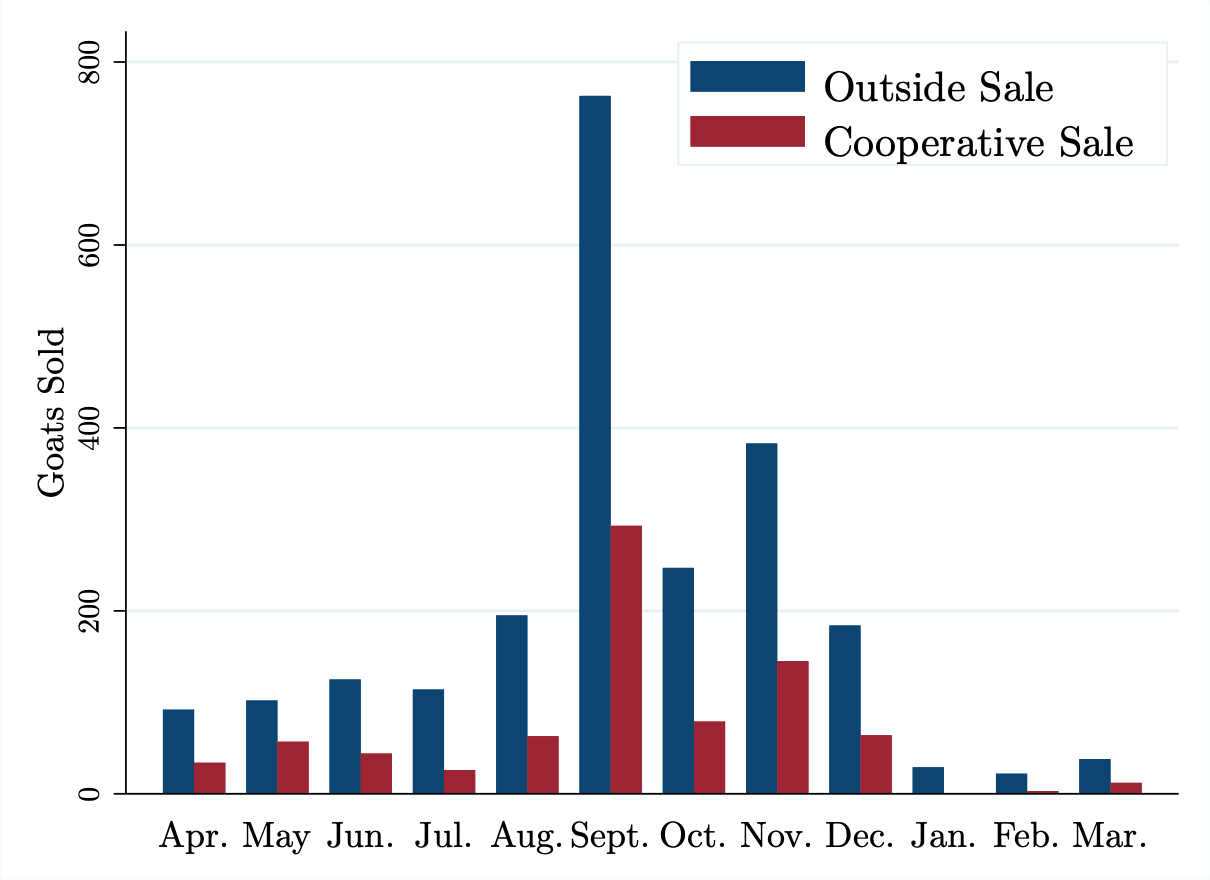
\includegraphics[width=.55\textwidth,trim=4 4 4 4,clip]{E2_SaleMonth.png}
\end{figure}

Figures (\ref{figure:E2_PD_Annual}-\ref{figure:E2_PD_NonFest}) display the distribution of goat prices received through each sale channel for the full calendar year, during festival season and outside of festival season. These figures suggests that selling goats through the cooperative may be more lucrative than side-selling, regardless of the timing of the sale. This further motivates the empirical puzzle that I will investigate in this essay. 

\begin{figure}[H]
\caption{Distribution of Goat Prices by Sale Channel (2018 Sample)}
    \centering
    \begin{subfigure}[t]{.49\textwidth}
    \centering
        \caption{Annual} \label{figure:E2_PD_Annual}
        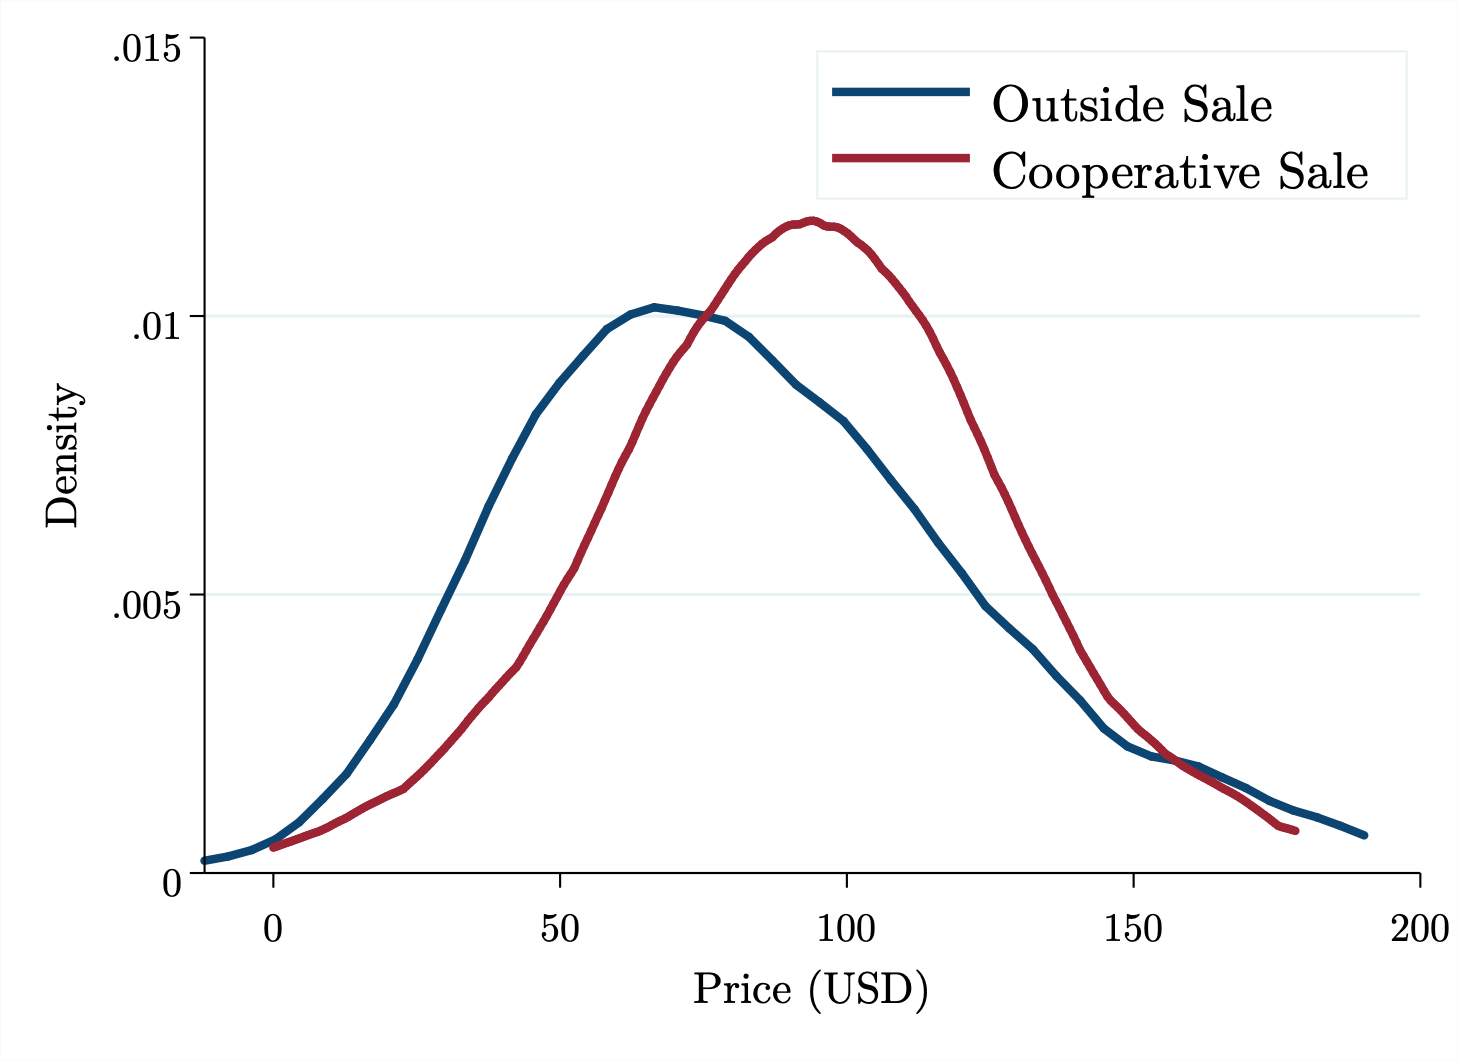
\includegraphics[width=\linewidth,trim=4 4 4 4,clip]{E2_PriceDensity_Annual.png} 
    \end{subfigure}
    \vspace{.5cm}
    \begin{subfigure}[t]{0.49\textwidth}
        \centering
        \caption{Festival Season} \label{figure:E2_PD_Festival}
        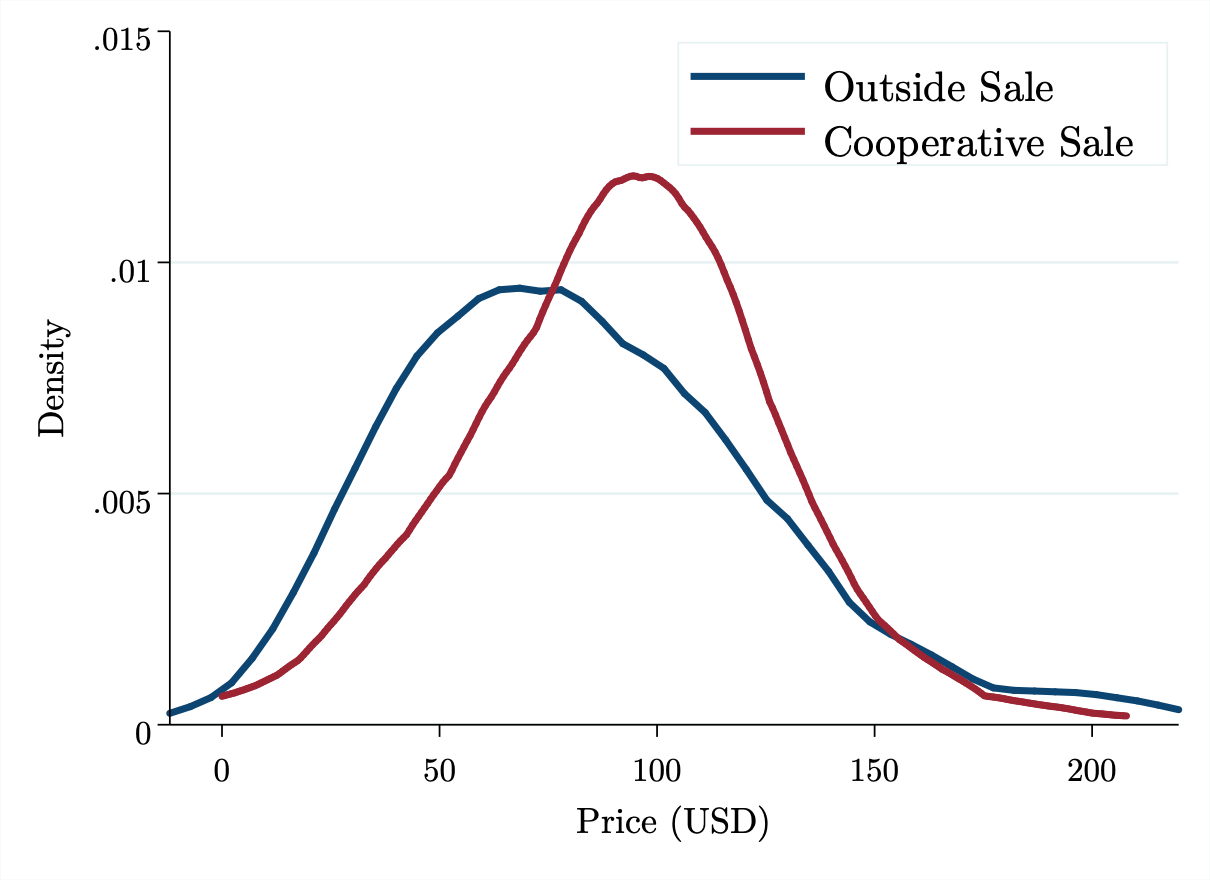
\includegraphics[width=\linewidth,trim=4 4 4 4,clip]{E2_PriceDensity_Festival.png} 
    \end{subfigure}
    \hfill
    \begin{subfigure}[t]{0.49\textwidth}
        \centering
        \caption{Non-Festival Season} \label{figure:E2_PD_NonFest}
        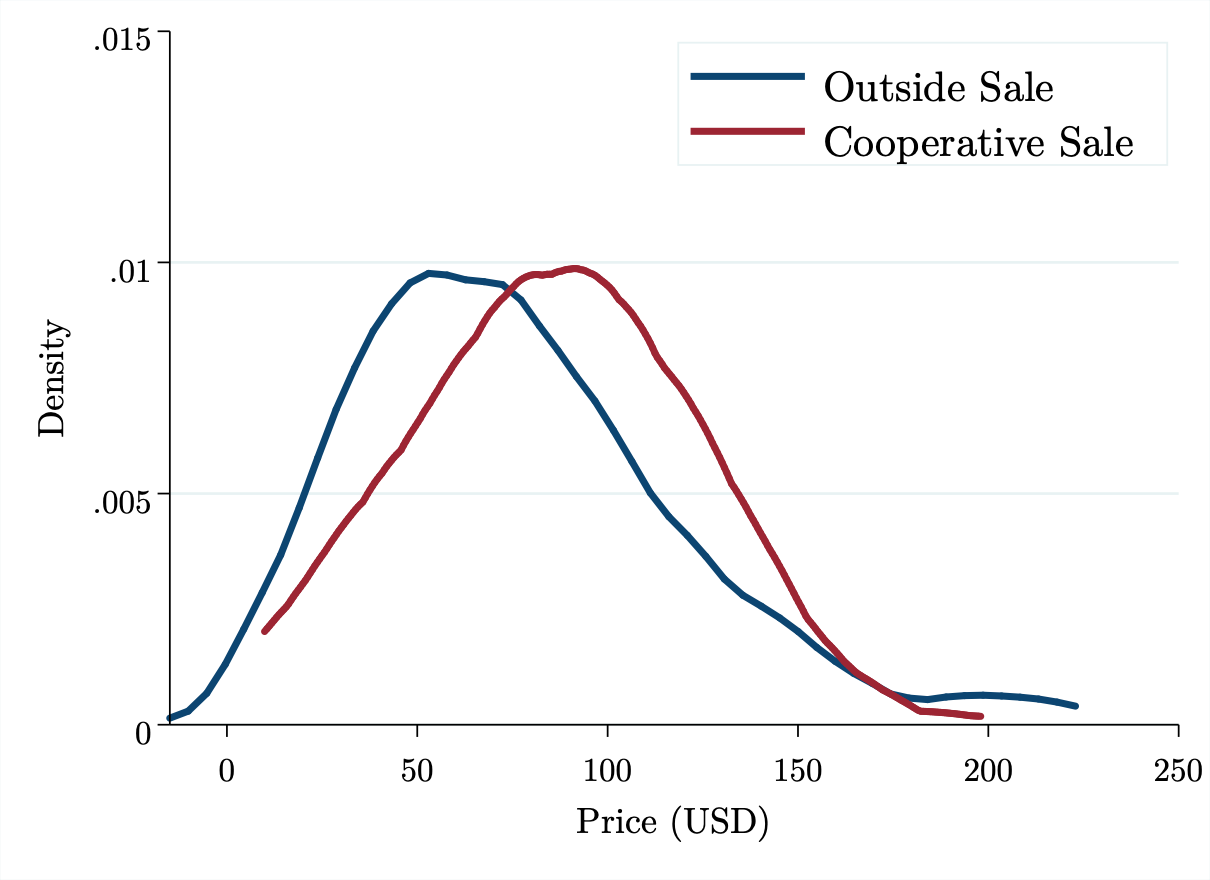
\includegraphics[width=\linewidth,trim=4 4 4 4,clip]{E2_PriceDensity_NonFest.png} 
    \end{subfigure}
\end{figure}


% --------------------------------------
\subsection{Theoretical Framework} \label{sec:E2_theory}
% rewrite text
Following \citet{michler-et.al.18} and \citet{suri11}, my goal is to estimate the distribution of returns to cooperative goat sales in order to understand if producers are self-sorting into cooperative and outside sales based on whether or not `adopting' is beneficial for them. In order to do this, I estimate the production function that underlies the decision to sell through or outside of the cooperative. I begin by treating the decision to sell through the cooperative as a technology that farmers are able to adopt. While this decision differs from typical agricultural technology adoption decisions, this methodology is useful for understanding the decision-making process around the source of goat sales in this context. Under this framework, producers are faced with the decision to `adopt' (sell through the cooperative), which provides the potential for a higher price and/or a larger number of goats sold, or `not adopt' (sell directly to a local trader), which can be viewed as the standard selling mechanism. The remainder of this subsection closely follows \citet{michler-et.al.18}, and the estimation will be conducted using the Stata package developed by \citet{cabanillas-et.al.18}.

I begin by using a Roy model which assumes that the adoption choice is part of a profit maximization decision, where returns are a function of input costs, output quality and prices. I assume the underlying production function to be Cobb-Douglas and written as
%CM: Consider writing it in log form right away

\begin{equation} \label{eq:E2_yield.C}
    Y^{C}_{it} = e^{\beta^{C}_{t}}\big{(}\prod_{j=1}^{k}X^{\gamma^{C}_{i}}_{ijt}\big{)}e^{u^{C}_{it}}
\end{equation}   
\begin{equation} \label{eq:E2_yield.O}    
    Y^{O}_{it} = e^{\beta^{O}_{t}}\big{(}\prod_{j=1}^{k}X^{\gamma^{O}_{i}}_{ijt}\big{)}e^{u^{O}_{it}}
\end{equation}

%CM: define your subscripts
where $Y^{C}_{it}$ and $Y^{O}_{it}$ are the quantity of goats sold through the cooperative (C) and outside of the cooperative (O), respectively. Yields are a function of inputs ($X^{\gamma^{O}_{i}}_{ijt}$), which can have differential effects on output depending on the adoption decision ($\gamma^{C}_{i}$ and $\gamma^{O}_{i}$). The $\beta$’s are adoption-specific aggregate returns to production, and the $u^{C}_{it}$ and $u^{O}_{it}$ terms are adoption-specific compound error terms, such that

\begin{equation} \label{eq:E2_u.C}
    u^{C}_{it} = \theta^{C}_{i} + \varepsilon^{C}_{it}
\end{equation}
\begin{equation} \label{eq:E2_u.O}
    u^{O}_{it} = \theta^{O}_{i} + \varepsilon^{O}_{it}
\end{equation}

Following \citet{carniero-et.al.15}, \citet{michler-et.al.18} and \citet{suri11}, I assume that households know their own farmer-specific productivity effects, $\theta^{C}_{i}$ and $\theta^{O}_{i}$, but do not know $\varepsilon^{C}_{it}$ and $\varepsilon^{O}_{it}$ prior to the sale. I also assume $\varepsilon^{C}_{it}$ and $\varepsilon^{O}_{it}$ to be uncorrelated with each other as well as with the $X$’s.
As in \citet{lemueux.98}, since $\theta^{C}_{i}$ and $\theta^{O}_{i}$ are unobserved, they can be decomposed into the following productivity effects %CM: The decomposition in 14 and 15 just redefines the variables as a regression. You can write anything as a regression on anything with a zero mean error. Also the thetas have to be mean zero, right? Otherwise you'd have an intercept.

\begin{equation} \label{eq:E2_theta.C}
    \theta^{C}_{i} = b_{C}(\theta^{C}_{i} - \theta^{O}_{i}) + \zeta_{i}
\end{equation}
\begin{equation} \label{eq:E2_theta.O}
    \theta^{O}_{i} = b_{O}(\theta^{C}_{i} - \theta^{O}_{i}) + \zeta_{i}
\end{equation}

where the projection coefficients $b_{C}$ and $b_{O}$ are defined as \singlespacing
$$b_{C} = (\sigma^{2}_{C} - \sigma_{CO}) / (\sigma^{2}_{C} + \sigma^{2}_{O} - \sigma_{CO})$$ 
$$b_{O} = (\sigma^{2}_{O} - \sigma_{CO}) / (\sigma^{2}_{C} + \sigma^{2}_{O} - \sigma_{CO})$$
$$\sigma^{2}_{C} \equiv Var(\theta^{C}_{i})$$
$$\sigma^{2}_{O} \equiv Var(\theta^{O}_{i})$$
$$\sigma_{CO} \equiv Cov(\theta^{C}_{i},\theta^{O}_{i})$$
\doublespacing
%CM: shouldn't b_{O} have -1*(\sigma^{2}_{O} - \sigma_{CO}) in its numerator? 

The $\zeta_{i}$ is a household’s absolute advantage in agricultural production and thus does not vary by the adoption decision.
I then define $\phi \equiv b_C / b_O - 1$ and rewrite equations (\ref{eq:E2_theta.C}) and (\ref{eq:E2_theta.O}) as

\begin{equation} \label{eq:E2_theta2.C}
    \theta^{C}_{i} = (\phi + 1)\theta_{i} + \zeta_i
\end{equation}
\begin{equation} \label{eq:E2_theta2.O}
    \theta^{O}_{i} = \theta_{i} + \zeta_i
\end{equation}

where $\theta_{i} \equiv b_{O}(\theta^{C}_{i} - \theta^{O}_{i})$. Equation (\ref{eq:E2_theta2.C}) relates the productivity of a household in cooperative sales $\theta^{C}_{i}$ to the household’s comparative advantage in cooperative sales compared to outside sales $\theta_{i}$ and the household’s absolute advantage in goat production $\zeta_i$. Additionally, $\phi$ is a measure of how important comparative advantage is for cooperative sales. The goal of this procedure is to empirically estimate the structural parameter $\phi$ and the distribution of $\theta_{i}$.
%CM: $\phi$ as a measure of comparative advantage could be made  more intuitive. Can you give us a clear explanation as to why it captures comparative advantage? 

I now rewrite the original Cobb-Douglas functions after taking logs to linearize the equations and replace the $u^{C}_{it}$ and $u^{O}_{it}$ with their decompositions:

\begin{equation} \label{eq:E2_y.C}
    y^{C}_{it} = \beta^{C}_{t} + X^{\prime}_{it}\gamma^{C}_{j} + (\phi + 1)\theta_{i} + \zeta_i + \varepsilon^{C}_{it}
\end{equation}
\begin{equation} \label{eq:E2_y.O}
    y^{O}_{it} = \beta^{O}_{t} + X^{\prime}_{it}\gamma^{O}_{j} + \theta_{i} + \zeta_i + \varepsilon^{O}_{it}
\end{equation}

Using a generalized yield equation of the form $y_{it} = h_{it}y^{C}_{it} + (1-h_{it})y^{O}_{it}$ and substituting in equations (\ref{eq:E2_y.C}) and (\ref{eq:E2_y.O}), I can define my empirical specification as

\begin{equation} \label{eq:E2_spec}
    \begin{split}
    y_{it} = & \beta^{O}_{t} + X^{\prime}_{it}\gamma^{O}_{j} + (\beta^{C}_{t} - \beta^{O}_{t})h_{it} +  X^{\prime}_{it}(\gamma^{C}_{j} - \gamma^{O}_{j})h_{it} \\
    & + \theta_{i} + \phi\theta_{i}h_{it} + \zeta_i + \varepsilon_{it}
    \end{split}
\end{equation}

where $h_{it}$ is the decision by household $i$ at time $t$ to sell through the cooperative and $\varepsilon_{it} \equiv h_{it}\varepsilon^{C}_{it} + (1-h_{it})\varepsilon^{O}_{it}$. Here, the coefficient $\phi\theta_{i}$ on the adoption term depends on the unobserved $\theta_{i}$ and is likely to be correlated with the adoption decision. Note that this model closely resembles a households fixed effects model, but relaxes a key assumption that limits the fixed effects approach. If I were to restrict $\phi = 0$ so that comparative advantage had the same effect regardless of adoption decision, this would be equivalent to the household fixed effects model \citep{suri11}. The major drawback of the fixed effects approach is that it assumes that the (endogenous) adoption decision is actually independent of a household’s comparative advantage in adopting. The CRC model relaxes this assumption and allows the unobserved effect to vary by adoption choice.

I propose to estimate the distribution of comparative advantage in cooperatives sales, $\theta_i$, and how important this comparative advantage is, $\phi$, which describes the sorting of households into cooperative and outside sales \citep{michler-et.al.18}. If $\phi > 0$, the sorting process leads to greater inequality in returns as households with relatively high levels of comparative advantage sell through the cooperative and see increasing gains from doing so. If $\phi < 0$ would imply that cooperative sales will still be optimal for households with relatively small levels of comparative advantage. If $\phi = 0$, a household’s comparative advantage is not important for the decision to sell through or outside of the cooperative.

% --------------------------------------
\subsection{Empirical Strategy} \label{sec:E2_emp}

\subsubsection{Identification of the Yield Function}

Identification of equation (\ref{eq:E2_spec}) requires two assumptions \citep{michler-et.al.18,suri11}. The first is mean independence of the composite error and unobserved comparative advantage terms and the exogenous regressors. This amounts to

\begin{equation} \label{eq:E2_assumption1}
    E[\zeta_i + \varepsilon_{it} | \theta_{i}; h_{i1}, \dots, h_{iT}; X_{i1}, \dots, X_{iT}] = 0
\end{equation}

By differencing out $(\theta^{C}_{i} - \theta^{O}_{i})$, $\zeta_i$ is independent of $\theta_i$ (Heckman and Honore 1990; Suri 2011). The second assumption is strict exogeneity of the error term, which implies that transitory shocks do not affect the household’s adoption decision. In the case of livestock marketing cooperatives, the decision to sell through or outside of the cooperative likely happens after all production decisions have been made and goats have met a threshold weight and size. This requires that I take additional steps to rule out the influence of transitory shocks on adoption decisions. There are several possible ways in which a shock to the household can influence the adoption decision. For example, a household may experience a financial shock (such as an earthquake, a death in the family, etc.) that requires the household to liquidate assets in the form of livestock. In this scenario, the household may be willing to sell outside of the cooperative at a lower price in order to immediately receive cash. My data includes several variables that indicate whether the household has experienced such a shock. I will control for these variables as a means of accounting for these shocks.


% --------------------------------------
\subsubsection{Estimating the CRC Model} \label{sec:E2_est}

To estimate equation (\ref{eq:E2_spec}) I use \citeauthor{suri11}'s (\citeyear{suri11}) generalization of the correlated random effects (CRE) model \citep{chamberlin84}, and implemented into a Stata package by \citet{cabanillas-et.al.18}. Here, I outline the estimation procedure for a model without covariates, following \citet{michler-et.al.18} and \citet{suri11}. Assuming a data generating process that is given by

\begin{equation} \label{eq:E2_data.gen}
    y_{it} = \delta +  \beta h_{it} + \theta_{i} + \phi\theta_{i}h_{it} + \xi_{it}
\end{equation}

where $\xi_{it} \equiv \zeta_i + \varepsilon_{it}$, $\beta \equiv \beta^{C}_{t} - \beta^{O}_{t}$, and all other terms are as previously defined. Note that the problem in estimating this equation comes from the fact that both $h_{it}$ and $\theta_{i}$ are present in multiple places in the equation. As with the \citet{chamberlin84} CRE model, I estimate the $\theta_{i}$’s with their linear projection on the history of the household’s adoption decisions

\begin{equation} \label{eq:E2_theta.proj}
    \theta_{i} = \lambda_{0} +  \lambda_{1}h_{i1} + \lambda_{2}h_{i2} + \lambda_{3}h_{i1}h_{i2} + v_i
\end{equation}

Substituting equation (\ref{eq:E2_theta.proj}) into equation (\ref{eq:E2_data.gen}) for each time period yields the following structural equations:

\begin{equation} \label{eq:E2_struc1}
    \begin{split}
    y_{i1} = (\delta + \lambda_0) + [\lambda_1(1 + \phi) + \beta + \phi \lambda_0]h_{i1} + \lambda_{2}h_{i2} \\
    + [\lambda_3(1 + \phi) + \phi \lambda_2]h_{i1}h_{i2} + v_i + \phi v_{i}h_{i1} + \xi_{i1}
    \end{split}
\end{equation}
\begin{equation} \label{eq:E2_struc2}
    \begin{split}
    y_{i2} = (\delta + \lambda_0) + \lambda_{1}h_{i1} + [\lambda_2(1 + \phi) + \beta + \phi \lambda_0]h_{i2} \\
    + [\lambda_3(1 + \phi) + \phi \lambda_1]h_{i1}h_{i2} + v_i + \phi v_{i}h_{i2} + \xi_{i1}
    \end{split}
\end{equation}

with corresponding reduced forms

\begin{equation} \label{eq:E2_red1}
    y_{i1} = \delta_1 + \gamma_{1}h_{i1} + \gamma_{2}h_{i2} + \gamma_{3}h_{i1}h_{i2} + \eta_{i1}
\end{equation}
\begin{equation} \label{eq:E2_red2}
    y_{i2} = \delta_2 + \gamma_{4}h_{i1} + \gamma_{5}h_{i2} + \gamma_{6}h_{i1}h_{i2} + \eta_{i2}
\end{equation}

Equations (\ref{eq:E2_red1}) and (\ref{eq:E2_red2}) allow me to estimate the five structural parameters ($\lambda_1-\lambda_3,\beta,\phi$) from the six corresponding reduced form parameters ($\gamma_{1}-\gamma_{6}$). Note that with the normalization of the $\theta_{i}'s$ so that $\sum \theta_{i} = 0$, I eliminate $\lambda_0$. This gives the following restrictions on each structural parameter:

\begin{align*}
    \gamma_1 & = (1+\phi)\lambda_1 + \beta + \phi\lambda_0 \\
    \gamma_2 & = \lambda_2 \\
    \gamma_3 & = (1+\phi)\lambda_3 + \phi\lambda_3 \\
    \gamma_4 & = \lambda_1 \\
    \gamma_5 & = (1+\phi)\lambda_2 + \beta + \phi\lambda_0 \\
    \gamma_6 & = (1+\phi)\lambda_3 + \phi\lambda_1
\end{align*}

I estimate equations (\ref{eq:E2_red1})-(\ref{eq:E2_red2}) as seemingly unrelated regressions and preserve the six reduced form parameters in a vector $\boldsymbol{\pi}_{[6 \times 1]}$ and the variance-covariance matrices in a symmetric block matrix $\textbf{V}_{[6 \times 6]}$. The restrictions on the $\gamma$’s can be expressed as $\boldsymbol{\pi} = \textbf{H}\boldsymbol{\delta}$, where $\textbf{H}_{[6 \times 5]}$ embodies the six restrictions on $\gamma$, and $\boldsymbol{\delta}_{[5 \times 1]}$ is a vector of the five structural parameters. I then use the optimal minimum distance (OMD) function to estimate the structural parameters.%CM: you'll need to tell us what this is.


%-----------------------------------------------------------------------%
\newpage
\singlespacing
\section{The Impact of a Smartphone Marketing Application on Smallholder Livestock Producers in Nepal} \label{sec:E3}
\doublespacing

% --------------------------------------
\subsection{Motivation} \label{sec:E3_motivation}
Throughout the developed world, the rise of digital technology has transformed the economic landscape. Widespread access to information and communication technology (ICT) has provided the opportunity to solve critical market problems in a cost-effective and scalable way. This notion has been echoed by a rise in platforms such as Uber, Amazon and Alibaba that have greatly decreased transaction costs and expanded economic activity \citep{munger18}. By reducing the cost of coordination, these platforms increase the efficiency and profitability of economic transactions across a wide range of applications \citep{worldbank16}. Despite a dramatic increase in access to mobile technology throughout the developing world, similar digital platforms are not widespread in many low-income countries.

Mobile technology has the potential to play a significant role in efforts to alleviate poverty around the world \citep{aker-et.al.16}. This is especially true for rural households who largely depend on agriculture for their livelihoods. Smallholder agricultural producers, many of whom belong to cooperatives, struggle to access information, communicate with market actors and arrange sales. This leads to high transaction costs, weak bargaining power and price dispersion that limit income growth and investment in productive assets \citep{staal-et.al.97}. Although previous literature has shown that access to mobile phones and mobile phone-based interventions can positively affect smallholder agricultural producers \citep{aker10,cole-fernando12,curtois-subervie14,jensen07,nakasone13}, little is known about the effects of introducing mobile phone-based applications designed to solve market problems and increase economic activity. Prior research on the effects of apps has been limited by low rates of smartphone ownership in the developing world, but the gap between rich and poor countries has substantially narrowed over the last decade \citep{worldbank16}. In particular, the rate of smartphone ownership in the developing world grew from 18\% in 2013 to 47\% by 2018, with much higher rates of ownership among individuals 35 years of age and younger \citep{pew18}. As technology increasingly reaches the world’s poor, can mobile phone-based applications be harnessed to facilitate economic activity and increase the incomes of smallholder agricultural producers?

In this essay, I propose to evaluate the effects of a smartphone-based information-sharing app for livestock producers known as the ``Virtual Collection Center'' (VCC). The VCC allows rank-and-file cooperative members to regularly update leadership on available goat inventory. Cooperative leaders use inventory information to negotiate bulk sales with traders, and then invite cooperative members to sales events through the app. By lowering barriers to communication in an environment characterized by rugged terrain and long travel times between population centers, the VCC has the potential to encourage market participation by cooperative members, thereby raising incomes. 

I will evaluate the effects of the VCC using a cluster-randomized control trial where treatment is assigned at the cooperative level. Cooperative members in the treatment group receive access to the VCC app as well as training on how to use it through Heifer Project International Nepal (HPIN). At the completion of the study in spring 2020, I will (i) estimate average intent-to-treat (ITT) effects of the intervention on cooperative and individual level economic performance and (ii) assess treatment effect heterogeneity.

% Antecedents
By facilitating communication and the flow of information, mobile technology has the potential to help alleviate poverty around the world \citep{aker-et.al.16}. Mobile technology could be particularly helpful for rural households who depend on agriculture for their livelihoods. Smallholder agricultural producers sometimes struggle to access information, communicate with market actors, and arrange sales, resulting in high transaction costs, weak bargaining power, and price dispersion that limit income growth and investment in productive assets \citep{staal-et.al.97}. The existing literature shows that mobile-phone adoption and mobile phone-based interventions can positively affect smallholder bargaining power, production, and prices received \citep{cole-fernando12,curtois-subervie14,muto-yamano09,nakasone13,shimamoto-et.al.15}, while also improving producer and consumer welfare and reducing waste by eliminating price dispersion across markets \citep{aker10,jensen07}. However, mobile technology for agricultural development has not been universally effective. In some cases, access to mobile phones or mobile phone-based information services has increased farmer knowledge without affecting prices received \citep{aker-ksoll16,camacho-conover11}, and in others impacts have been limited by low adoption \citep{fafchamps-minten12,muto-yamano09}. 

While there is a rich literature on the impact of mobile phone coverage and related interventions, smartphones are a fairly recent development in low-income countries. Existing studies of smartphone apps for agriculture tend to consist of small pilots rather than large randomized trials. Examples include \citet{eitzinger-et.al.19}, who discuss GeoFarmer, a cloud-based smartphone app that allows farmers to share information with other producers and experts, and \citet{saito-et.al.15}, who develop a decision-support application that helps farmers in Senegal improve fungicide applications. % The research most relevant to this study have largely focused on increasing access to information and providing digital tools for farm management, . Weld et al. (\citeyear{weld-et.al.18}) design a mobile phone-based business directory app, eKichabi, and demonstrate its feasibility, use and scalability. % xxx include other examples?e-kichabi is dumbphone so i took it out

% Value Added
I will make several contributions to the existing literature. First, I will provide evidence on the impact of a smartphone app designed to increase economic activity in a rural area of a developing country. In addition, I add to the evidence on business development for woman entrepreneurs, smallholder livestock producers, and agricultural cooperatives. To my knowledge, there are no existing randomized control trial evaluations of business development for agricultural cooperatives. 

% --------------------------------------
\subsection{Background} \label{sec:E3_background}

The cooperatives included in this evaluation appear to struggle with coordinating goat sales in a way that is broadly inclusive of members. Although officers from 90 of the 92 cooperatives included in this study stated in baseline interviews that their organizations coordinated group sales, 43\% of households who had sold at least one goat in the 12 months prior to baseline data collection indicated that their cooperatives did not perform this service. 

Despite growth in mobile phone ownership, my baseline data suggest that the cooperatives studied here largely communicate in person. Less than 30\% of households in my sample received any information about sales organized through the cooperative in the 6 months prior to data collection. Among the households that did receive price and sales information, half indicate that they did so by word of mouth, nearly 75\% indicate receiving this information through SHG meetings, while only 19\% have received sales and price information by phone call and less than 1\% via short message service (SMS). The responses of rank-and-file cooperative members regarding use of mobile phones are reinforced by a survey of cooperative officers, who indicate that they contacted SHGs by SMS less than once and by phone call only three times in the month prior to data collection, on average. 

The failure to transmit information about sales could be the result of meeting infrequently, as nearly all households state that SHG meetings happen monthly or less while nearly two-thirds indicate that cooperative meetings take place every two months or less. Distance to meetings points could be a barrier to more frequent interactions, as cooperative members state that it takes approximately 75 minutes to travel to cooperative meetings, on average. Road quality, access to transportation, and distance between cooperative members were identified by 90\%, 93\%, and 83\% of cooperative leaders, respectively, as limiting communication. Cooperatives may be responding slowly to market demand and potentially losing sales in the time it takes to communicate with members, while also failing to consider the entire inventory of animals at their disposal. % By introducing a digital platform that allows cooperatives to access inventory, communicate market information and internally arrange sales, this intervention has the potential to increase communication flow, economic activity and cooperative performance.

The necessary conditions for an effective smartphone-based marketing intervention appear to be in place in rural Nepal. Survey data collected from a representative sample of HPIN beneficiaries for a prior project show that at least 47\% of members in every SHG own a mobile phone \citep{janzen16-1}. % xxx we are dumb and did not ask for phone ownership in our baseline
More recent data from the Nepal Telecommunications Authority (\citeyear{NTA19}) show that the mobile phone penetration rate (the number of SIM cards in use) exceeds 132\% of the total Nepali population. Smartphone ownership in Nepal has grown by roughly 10 percentage points each year since the start of the decade and surpassed 50\% in 2018 \citep{nepalitelecom18}. Virtually all of the country except for mountainous areas has 2G or better network coverage, allowing for voice, SMS, and basic internet usage through mobile phones.\footnote{For example, see the \href{https://www.ncell.axiata.com/About-Us/Coverage}{coverage map} for major carrier Ncell.} 

The difficulties associated with word-of-mouth communication beg the question of why mobile phones do not play a larger role in cooperative marketing. One barrier may be the lack of specialized communication tools that reduce the time and cost of making calls and sending text messages. Given that cooperatives average about 500 members each, calling all members or confirming that all receive a text message may seem more onerous than holding a meeting. Network quality is also an issue, with 89\% of cooperative leaders in my baseline data indicating that mobile network coverage limits communication within the cooperative. But mobile network coverage and smartphone ownership are likely to continue increasing in Nepal at rapid rates, while infrastructure improvements and other investments needed to make face-to-face communication in rural areas easier may not be forthcoming. These circumstances might accurately describe many rural areas reliant upon agriculture, making the effectiveness of smartphone marketing tools in rural Nepal an important development question.

% --------------------------------------
\subsection{Research Design} \label{sec:E3_research.design}
\subsubsection{Intervention} \label{sec:E3_intervention}
The VCC app was designed by a research team, including members from the University of Florida, University of Georgia and Kansas State University, and HPIN, and programmed by Pathway Technology and Services, a Nepali software firm that also shared responsibility for training cooperatives in the use of the app with HPIN. The VCC app was completed and piloted in 2018. After initial technical difficulties, the app was rolled out in earnest to the treatment group in December 2018.  

The app, which requires an Android smartphone, was designed to be easy to use by producers who have basic literacy and are familiar with smartphones, but probably not able to use a complicated program. The intervention was designed so that only one member of each SHG needs to have the VCC app installed on her smartphone, while a single cooperative officer manages the data compiled from all SHGs. The person responsible for the app at the SHG level is known as the ``SHG manager'' while the cooperative officer managing the app at a higher level is known as the ``cooperative VCC manager'' (as opposed to the regular cooperative manager, which is a separate position in the cooperative leadership hierarchy). As of June 2019 all SHG managers and cooperative VCC managers had the app installed on a smartphone.

Figure \ref{fig:diagram} provides a description of how the VCC platform is used to organize sales within a given cooperative. In step 1, SHG members report the quantity of small, medium and large goats available for sale to the SHG manager. Goat weight classifications and their associated cutoffs are commonly known. The SHG manager enters inventory information into the VCC app, and the app automatically sends the information to a server managed by HPIN in step 2. Sending and receiving information through the app requires cell service or an internet connection. Information sent through the application is done so in SMS format. Information cannot be sent or received without cell service and is delayed until service is restored.

In step 3, the server compiles the data sent by each SHG into a database and a summary table is automatically created for each cooperative and sent to the cooperative VCC manager. The summary table lists the quantity of small, medium, and large goats available for sale in each SHG. In steps 4 and 5, cooperative leaders use inventory information to coordinate sales with local buyers. Once a sale has been arranged, the cooperative leaders select specific SHGs to participate in the sale based on the inventory data in the VCC app. Using the VCC app, the cooperative VCC manager notifies the SHG managers of the date, location, trader, number of animals by weight category, and price per animal for the arranged sale in step 6. In step 7, the SHG manager confers with her fellow SHG members, and then lets the cooperative VCC manager know through the app how many members will attend the sale and the quantity of animals each will bring. If necessary, the cooperative VCC manager can invite additional SHGs until the buyer's order is filled. At the conclusion of the sale, the SHG manager enters updated information on the number of goats available into the VCC app, and the process begins again. In addition to inventory and sales coordination, the VCC app has a general-purpose messaging tool.

Figure \ref{fig:app} displays select images of the VCC interface that SHG managers see on their mobile device. The left-most image depicts the home screen, where users can navigate the various functions of the app. The center image displays the screen where SHG managers update the quantity of available goats within the SHG. The right-most image depicts sale information that is sent to an SHG manager if her SHG is invited to a sale.

\newpage

\begin{figure}[!h]
    \caption{VCC Network Diagram}
    \label{fig:diagram}
    \noindent \centering 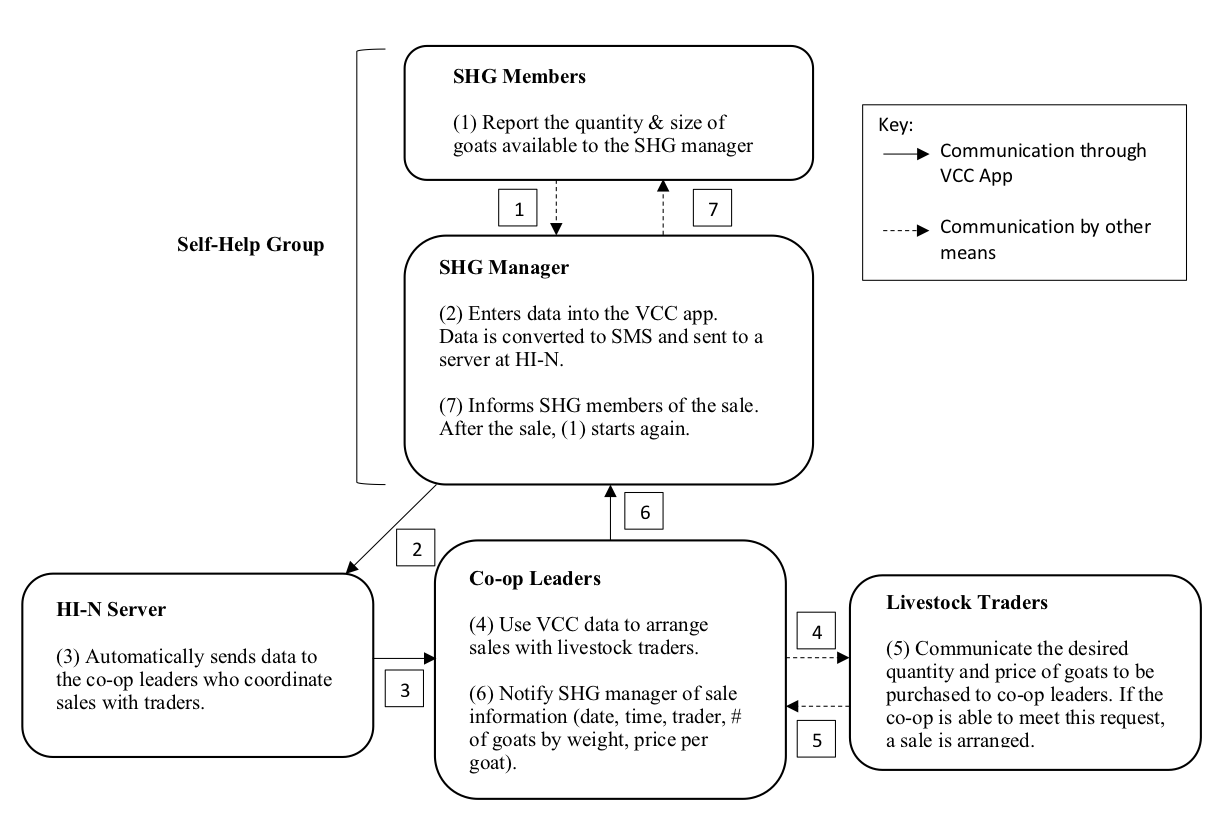
\includegraphics[width=.8\textwidth]{VCCdiagram.png}
\end{figure}

\begin{figure}[!h]
  \caption{VCC Application Interface}
  \label{fig:app}
  \begin{minipage}{.2\textwidth}
    
\includegraphics[width=6cm]{vcc1.png}
  \end{minipage}
  \hspace{1.5cm}
  \begin{minipage}{.2\textwidth}
    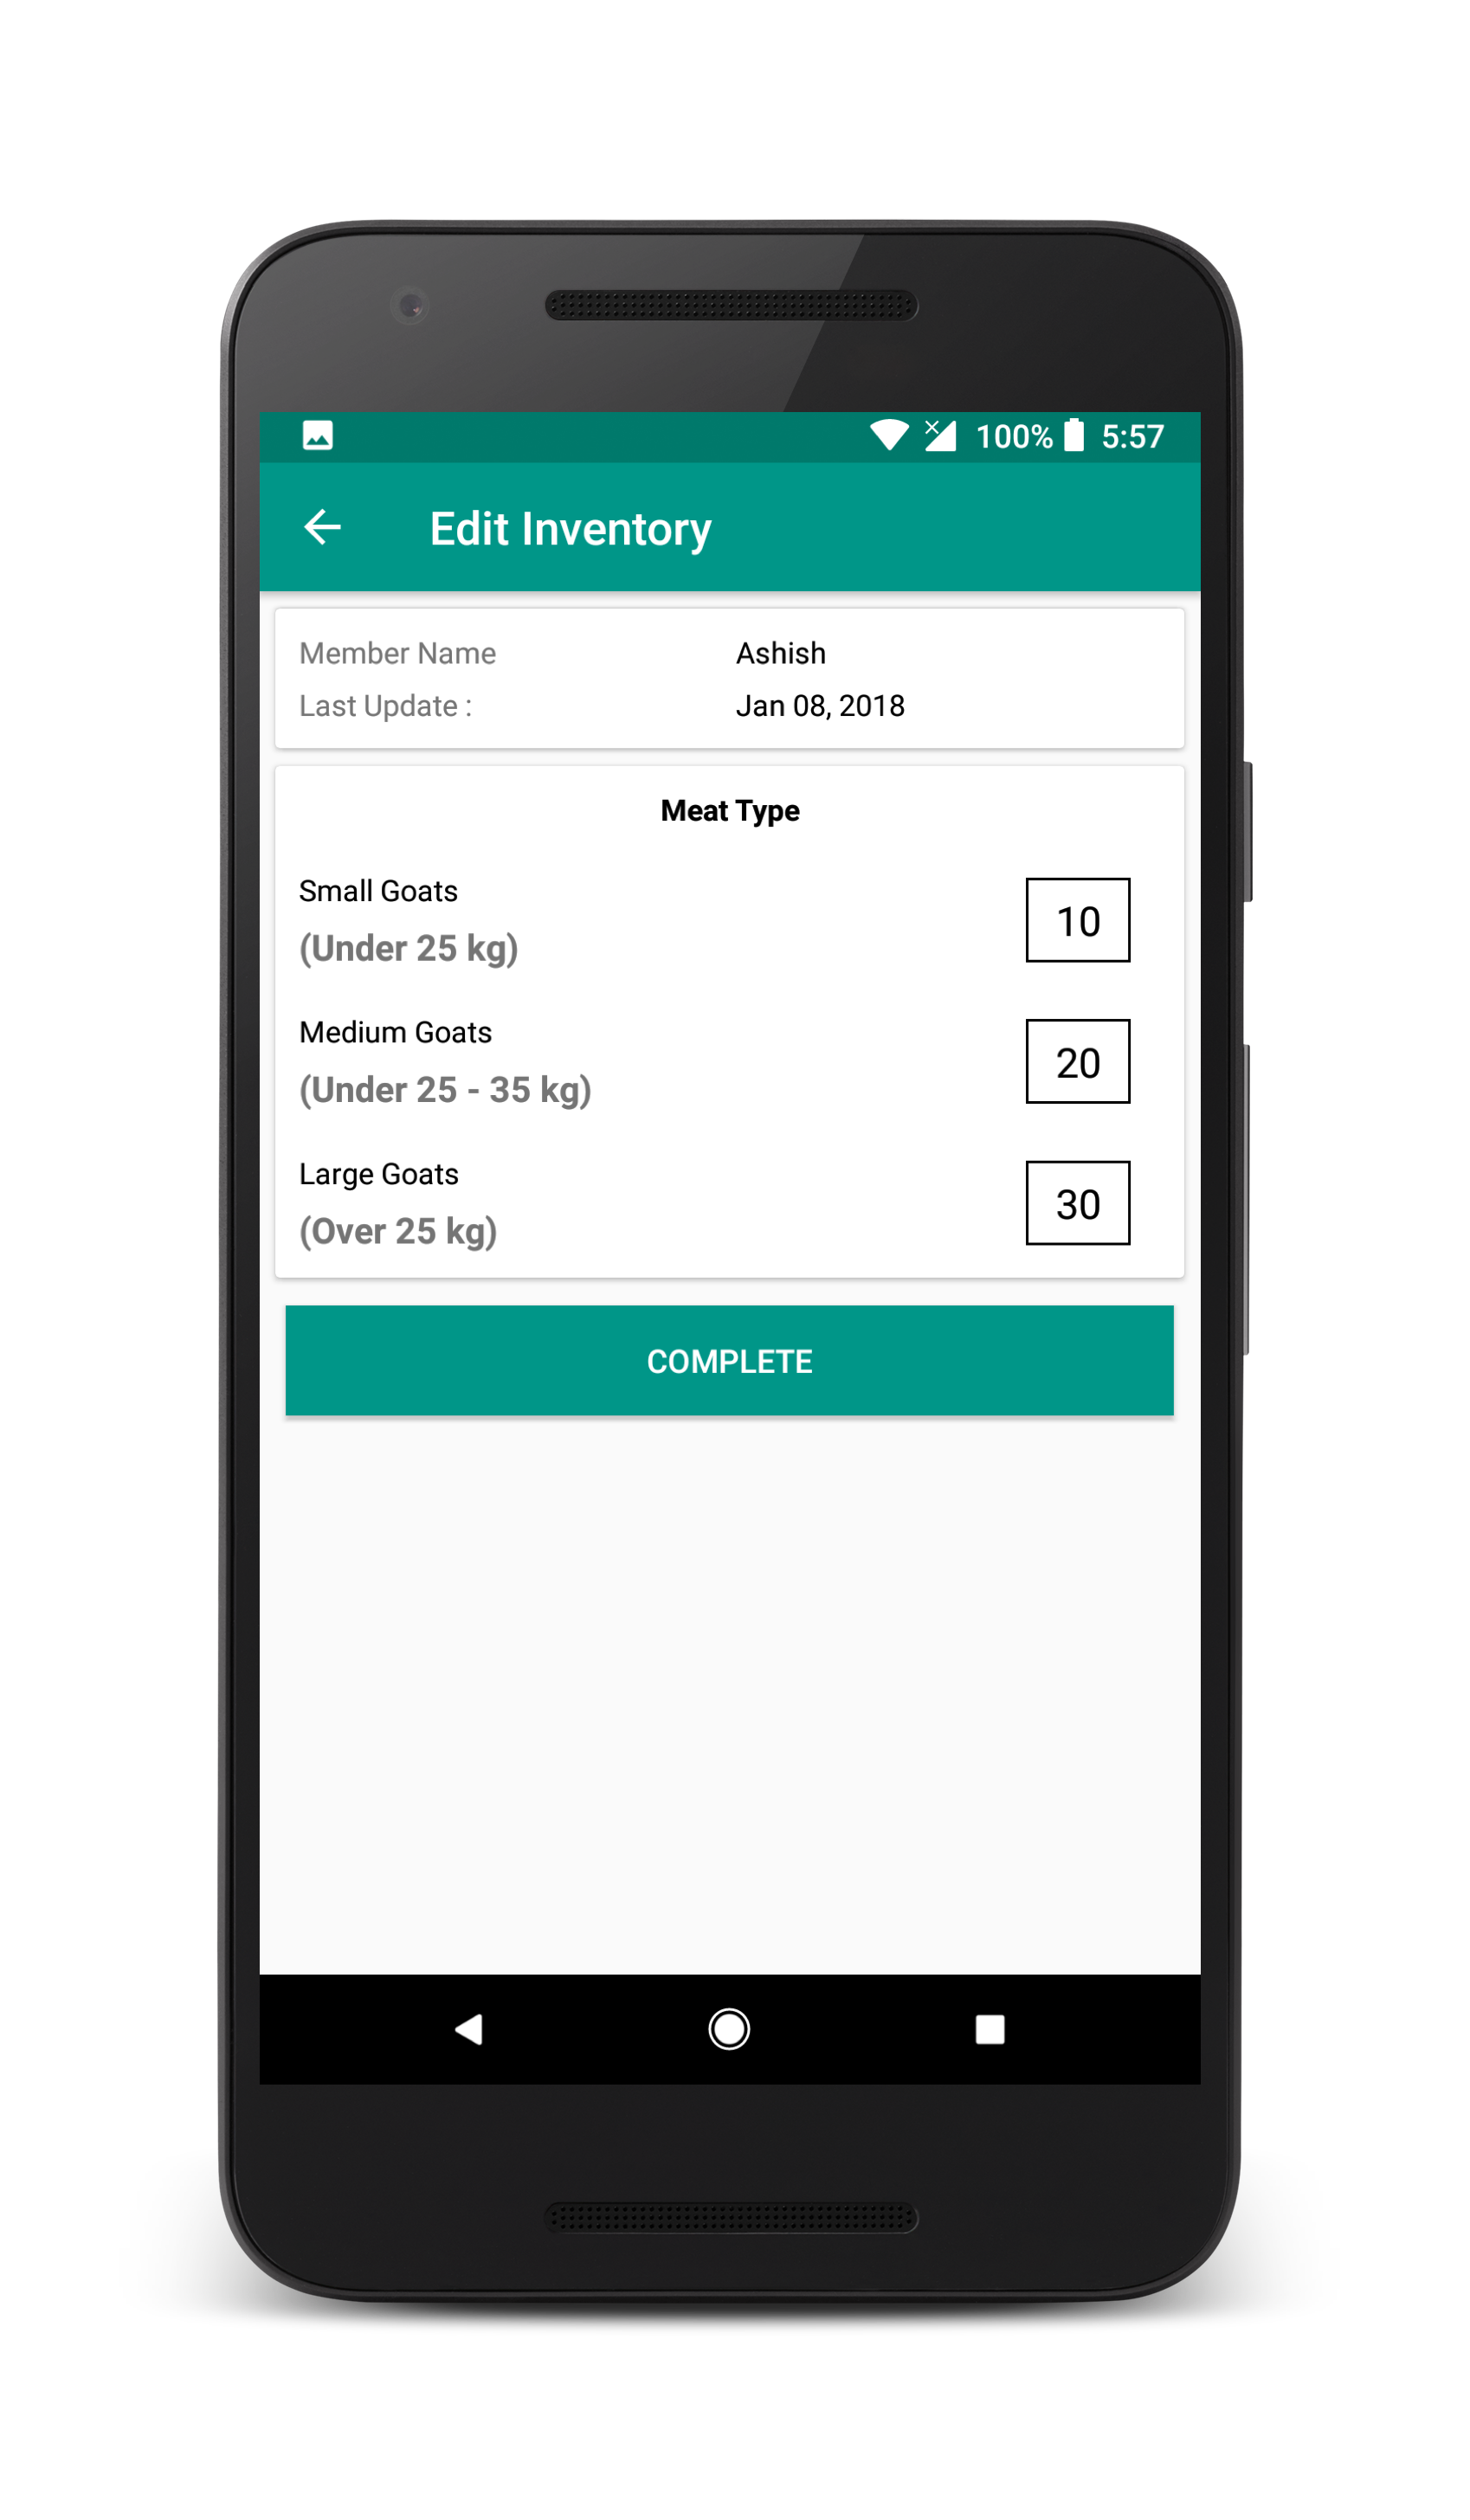
\includegraphics[width=6cm]{vcc2.png}
  \end{minipage}
  \hspace{1.5cm}
  \begin{minipage}{.2\textwidth}
    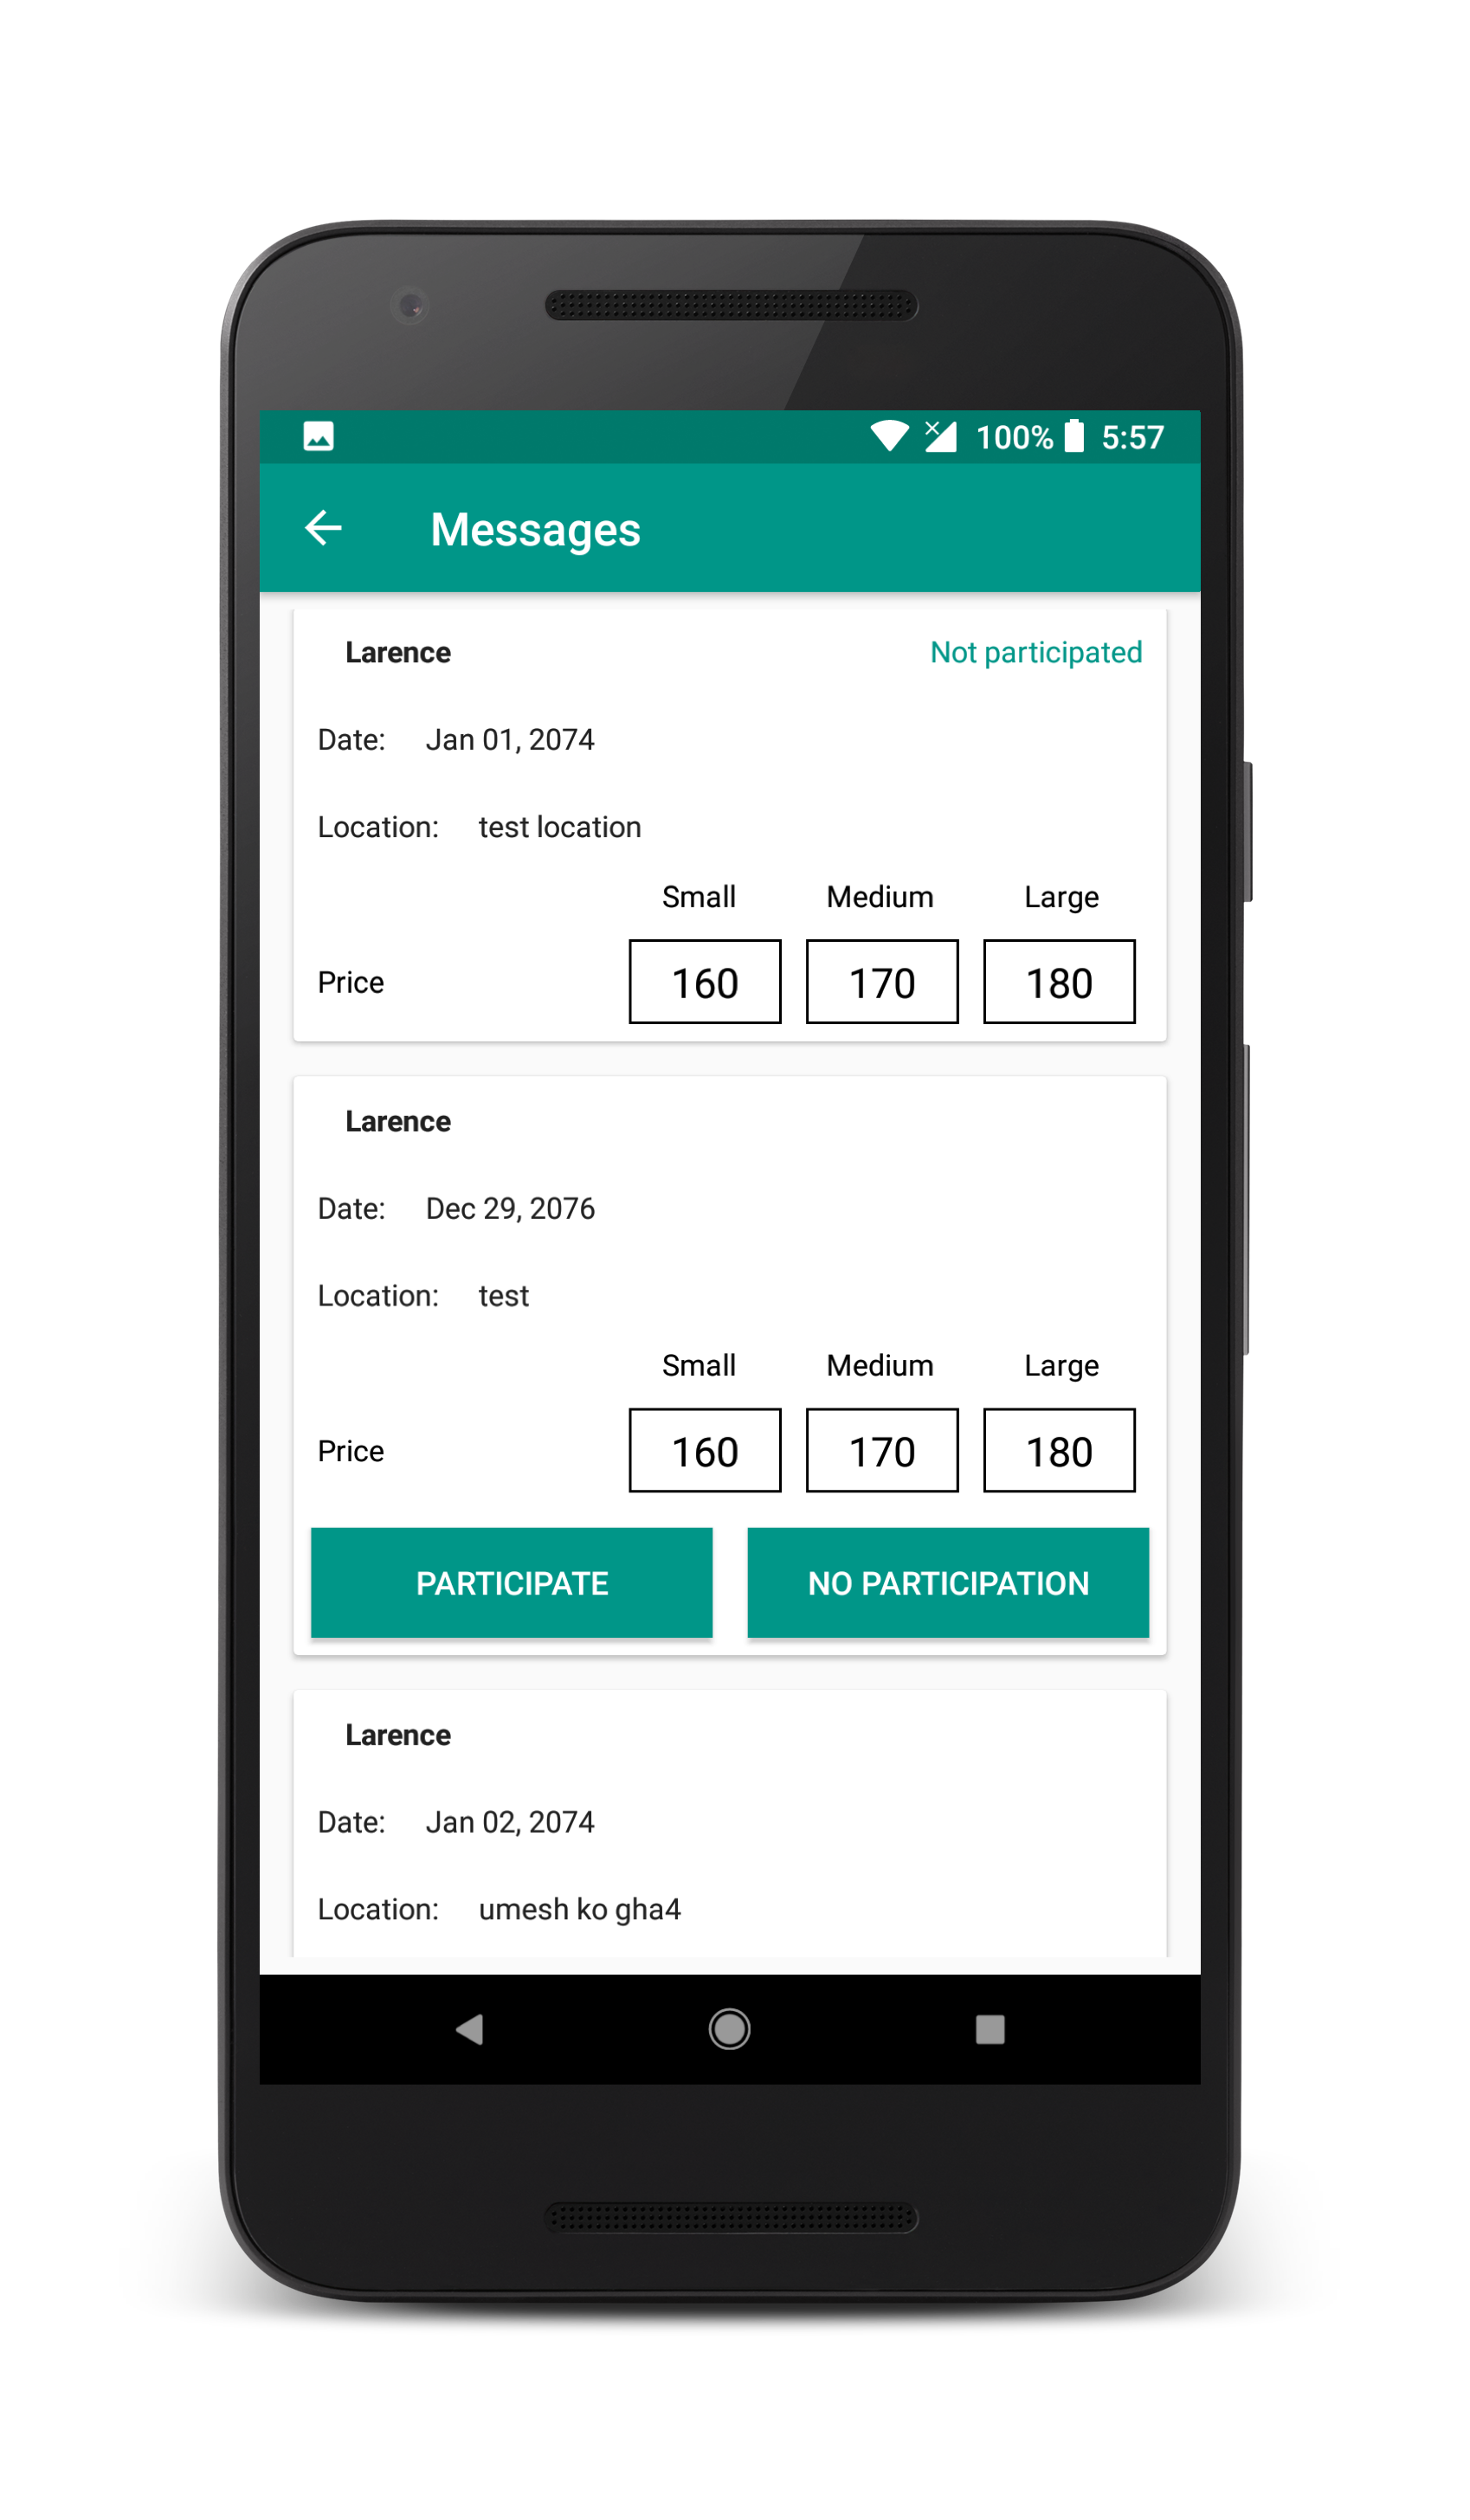
\includegraphics[width=6cm]{vcc3.png}
  \end{minipage}
\end{figure}

\newpage


% --------------------------------------
\vspace{2cm}
\subsubsection{Experimental design} \label{sec:E3_experimental.design}

The impact of the VCC platform will be evaluated using a cluster RCT spanning 91 cooperatives in Nepal. Treatment was assigned at the cooperative level through a stratified randomization design as described in detail in section \ref{sec:E3_assignment}.  Treatment effects will be estimated at both the household and cooperative levels. 

Cooperatives cover a wide geographic area.  Based on conversations with HPIN, we understand cooperatives largely sell to local markets and buyers, such that broader macroeconomic price impacts (extending beyond the geographic borders within which the cooperative operates) are not anticipated. Cooperatives are geographically based, and members of a cooperative are only able to sell through their cooperative. Because cooperative membership comes through SHG membership, and SHG membership is extremely local (tole, or neighborhood), non-members would only be able to join their local cooperative and not a cooperative in a different treatment group. 


\subsubsection{Research questions} \label{sec:E3_hypothesis}
My study will answer the following questions: (i) across a range of dimensions of cooperative performance (measured at the cooperative and household levels), what are the overall impacts of access to the VCC, (ii) are the effects of the VCC heterogeneous, and if so, (iii) how do the households and cooperatives most and least affected by the intervention compare in terms of their observed characteristics?

If effective, the VCC app could transform households and cooperatives in our study area as follows. By improving access to market information and reducing the costs of coordination within cooperatives for group marketing, I hypothesize that the VCC application will increase the proportion of cooperative members made aware of cooperative-organized sales. More generally, the improved flow of communication stimulated by the VCC app may make cooperatives more transparent, where transparency is measured by how closely aligned management and rank-and-file members are in their responses to questions about the services offered by their cooperative.
%NM: "Transform" is a strong word. I think going after transparency is a bad idea, at least as a primary outcome. 
Improved awareness of group sales will raise the quantity of goats sold through cooperatives and the total number of goats sold overall. Raising the number of goats sold through cooperatives may have two impacts on prices received: first, by selling more goats through cooperatives, households may receive higher prices, and second, selling more goats through cooperatives may increase cooperative bargaining power by limiting side selling, leading to higher prices received for goats sold through cooperatives. The combination of selling more goats and doing so at higher prices will lead to increased net goat income at the household level. 
%NM: What about higher prices from selling by weight?
The VCC app may also transform cooperative management. As demonstrated by \citeauthor{lajaaj.17} (\citeyear{lajaaj.17}) using randomized assignment of input subsidies and matched savings to rural households in Mozambique, poverty shortens planning time horizons. Similarly, I hypothesize that improved cooperative performance will translate into longer planning time horizons for cooperative leaders, as well as higher expectations for future goats sold and revenue. %NM: I think Lajaaj isn't a good comparison. The longer time horizon might not be from the ability to see a better future, but from the ability to plan. Also, how coop leaders see the future and why they see it how they do is likely different for individuals (for themselves) and coop leaders (for their coops).

Below I organize my hypothesized effects of the VCC app into five research questions. Each research question has a corresponding family of hypothesis tests where I will test the null of no effect on the outcomes listed below each question. For a given research question, I will answer in the affirmative if I reject the null hypothesis of no effect for at least one associated outcome while adjusting for multiple hypothesis testing. Note that the outcomes used to answer questions 2, 3, and 4 overlap because of my approach to adjusting for multiple hypothesis testing, which I describe in section \ref{sec:E3_mult.inf}. 

\singlespacing
\begin{itemize}
    \item \textbf{Question 1:} Does access to the VCC application improve communication within cooperatives?
        \begin{enumerate}
        % \item[1a)] Number of times members receive information about cooperative sales
        % \item[1b)] Number of times members receive information about cooperative activities
        % \item[1c)] Communication Summary Index
            \item[1a)] Household is aware that their cooperative organizes goat sales with traders (0/1)
            \item[1b)] Household contacted at least once about cooperative goat sale in past 12 months (0/1)
            \item[1c)] Transparency index
        \end{enumerate}
    
    \item \textbf{Question 2:} Does access to the VCC application increase goat sales?
        \begin{enumerate}
        % \item[2a)] Household goats sold
        % \item[2b)] Household goat revenue
        % \item[2c)] Household goats sold through cooperative
        % \item[2d)] Household goat revenue through cooperative
        % \item[2e)] Household net goat income
        % \item[2f)] Goat Sales Summary Index
            \item[2a)] Number of goats sold by the household through the cooperative (count)
            \item[2b)] Number of goats sold by the household (count)
        \end{enumerate}
    
    \item \textbf{Question 3:} Does the VCC application increase prices received for goats?
        \begin{enumerate}
            \item[3a)] Revenue per goat sold (USD)
            \item[3b)] Revenue per goat sold through the cooperative (USD)
        \end{enumerate}
    
    \item \textbf{Question 4:} Does the VCC application increase net household goat income?
        \begin{enumerate}
            \item[4a)] Revenue per goat sold (USD)
            \item[4b)] Number of goats sold by the household (count)
            \item[4c)] Net household goat income (USD) 
        \end{enumerate}
%NM: Question 3 and 4 seem too similar. I understand there are some subtle differences, but think those differences make 4 a noisier version of 3 if 3 comes from individual data.
    \item \textbf{Question 5:} Does access to the VCC application improve the planning horizon and expectations of cooperative leaders?
    \begin{enumerate}
        \item[5a)] Planning time horizon (years)
        \item[5b)] Number of goats expected to be sold through cooperative in next six months (count)
        \item[5c)] Total revenue expected to be earned by cooperative in next six months (USD)
%NM: Planning horizon does merit some explanation. I worry revenue expected is going to be difficult to capture and have wild estimates.
    \end{enumerate}
\end{itemize}
\doublespacing

Most outcomes are self-explanatory. The lone exception is the ``transparency index''. My data set contains seven binary variables that indicate whether the cooperative general manager states that the cooperative makes certain information available to its members. I also asked each cooperative member household in my sample the same questions. The index is created by coding disagreements between the cooperative manager as zeroes and agreements as ones. The resulting variables are then combined into an inverse covariance weighted index as described in \citeauthor{anderson08} (\citeyear{anderson08}). 

% --------------------------------------
\subsection{Data} \label{E3_data}

% --------------------------------------
\subsubsection{Assignment to treatment} \label{sec:E3_assignment}
To form strata prior to randomization, I first used the baseline data from both the household and cooperative leader survey to identify what I expect to be strong predictors of my outcomes of interest, including region (Terai and Mid-Hills), household goat revenue over the past 12 months, number of cooperative members, and cooperative revenue. Household goat revenue was top coded, replacing obvious outliers with reported number of goats sold multiplied by the median revenue per goat sold. The strata were then created using the following steps:
  \begin{enumerate}
  	\item Dropping a single cooperative that was used in a pilot of the VCC app, leaving 108 cooperatives in total.
    \item Sorting cooperatives within each region by average household-level goat revenue.
    \item Splitting each region at its 33\textsuperscript{rd} and 66\textsuperscript{th} percentiles of average household goat revenue, yielding six bins.
    \item Sorting cooperatives in each of the six bins by number of cooperative members.
    \item Splitting each bin at the median number of cooperative members, yielding a total of 12 bins.
    \item Sorting each of the 12 bins by cooperative revenue.
    \item Splitting each bin at the median of cooperative-level revenue (from any source), yielding a total of 24 bins ranging in size from four to six cooperatives. 
  \end{enumerate}

Within each cooperative, I generated a uniform random variable and assigned the two (in the case of strata with four or five members) or three (in the case of strata with six members) cooperatives with the greatest value of the random variable to treatment. For strata with five members, the odd-numbered cooperative was assigned to treatment with 50\% probability using a uniform random variable. 

A complications arose around the time of treatment assignment. HPIN informed the research team that cooperatives in a single district could not be part of the randomization because the cooperatives work together to market goats. At that point, the randomization was complete and cooperatives had already been contacted to coordinate VCC app training. Therefore it would have been problematic to perform the randomization again. Instead, I verified that balance for my chosen indicators was maintained after dropping the cooperatives from the aforementioned district.\footnote{Cooperatives in this district union were removed from the research design but were allowed to proceed using the app.} The final treatment assignment includes 91 cooperatives in total, with 44 assigned to treatment and 47 assigned to control.


\subsubsection{Summary statistics and balance} \label{sec:E3_summary}
The summary statistics displayed in table \ref{table:E3_summary.stats} demonstrate that cooperatives in my sample vary in both size and economic activity. The average cooperative has over 500 members and revenue of nearly \$3,800 USD. Total membership ranges from 11 to 2,600 while cooperative revenue ranges from \$0 to over \$65,700 USD. I observe similar variation across cooperative members. The average household sold one goat in the past year, and received \$42 USD in revenue per goat sold. Note that revenue per goat was set to zero for households not selling any goats, making revenue per animal (especially for sales through cooperatives) appear artificially low. Goats sold through the cooperative range from zero to 15, while the total number of goats sold range from zero to 24. 

Tables \ref{co.balance} and \ref{hh.balance} display balance across the treatment and control groups in the cooperative and household-level data. All outcomes of interest are balanced across treatment and control groups at baseline. 
% xxx were stratum dummies used in the balance tests? They probably should be, and if they were, please say so in the table notes. Please get rid of shorthand (HH) in tables and only capitalize first word of each variable name. Binary variables should be identified as such by a (0/1) at the end of their names, count variables with (count), monetary with (USD). 

%\newpage
\singlespacing
% Summary Stats Table
\newcolumntype{Y}{>{\centering\arraybackslash}X}
\begin{table}[!h]
  \centering
  \caption{Summary Statistics}
  \label{table:E3_summary.stats}
  \scalebox{.8}{
  \begin{tabularx}{\linewidth}{l*{7}{Y}}
\hline Cooperative-Level Variables & N & Mean & sd & Min & Max\\
\noalign{\smallskip}\hline \noalign{\smallskip}
Members (count) & 92 & 553.36 & 376.42 & 11.00 & 2,600.00\\
Revenue (USD) & 92 & 3,775.21 & 8,014.47 & 0.00 & 65,709.51\\
Costs (USD) & 92 & 377.52 & 1,639.07 & 0.00 & 10,964.25\\
Net revenue (USD) & 90 & 3,473.19 & 8,245.85 & -7,935 & 65,554.27\\
Revenue per member (USD) & 92 & 7.20 & 10.55 & 0.00 & 63.53\\
Net revenue per member (USD) & 90 & 6.80 & 10.95 & -13.22 & 63.53\\
Goat revenue (USD) & 90 & 111.86 & 203.73 & 0.00 & 1,029.40\\
Planning time horizon (years) & 92 & 1.26 & 0.98 & 0.00 & 5.00\\
Expected goats sold (count) & 92 & 269.09 & 359.69 & 0.00 & 2,500.00\\
Expected revenue (USD) & 92 & 1,011.83 & 2,136.93 & 0.00 & 14,850.00\\
Number of ICT assets (count) & 92 & 0.57 & 0.74 & 0.00 & 3.00\\
Number of non-ICT assets (count) \hspace{1.4cm} & 92 & 2.79 & 2.47 & 0.00 & 15.00\\


  \end{tabularx}}
  \scalebox{.8}{
  \begin{tabularx}{\linewidth}{l*{7}{Y}}
\hline Household-Level Variables & N & Mean & sd & Min & Max\\
\noalign{\smallskip}\hline \noalign{\smallskip}
Household has dirt floors (0/1) & 2,448 & 0.56 & 0.50 & 0.00 & 1.00\\
Household has more than one floor (0/1) & 2,448 & 0.58 & 0.49 & 0.00 & 1.00\\
Goat management index & 2,448 & 6.41 & 1.49 & 0.00 & 10.00\\
Goat empowerment index & 2,448 & 8.77 & 5.03 & 0.00 & 12.00\\
Age (years) & 2,448 & 42.82 & 11.72 & 6.00 & 83.00\\
Literacy (0/1) & 2,446 & 0.79 & 0.36 & 0.00 & 1.00\\
Number of SHG meetings attended (count) & 2,448 & 1.84 & 2.49 & 0.00 & 24.00\\
Received Sale Information (0/1) & 2,448 & 0.29 & 0.45 & 0.00 & 1.00\\
Goats sold through cooperative (count) & 2,448 & 0.22 & 0.75 & 0.00 & 5.00\\
Total goats sold (count) & 2,448 & 1.10 & 1.58 & 0.00 & 9.00\\
Revenue per goat sold (USD) & 2,448 & 42.10 & 49.84 & 0.00 & 193.05\\
Revenue per cooperative goat sold (USD) & 2,448 & 9.46 & 29.18 & 0.00 & 134.64\\
Net goat income (USD) & 2,448 & 59.15 & 138.82 & -276.21 & 696.96\\
Transparency discrepancy index & 1,647 & 0.31 & 1.05 & -1.14 & 2.11\\
\hline
\multicolumn{6}{@{}p{1\textwidth}}
{\textit{Notes}: Several variables have missing values replaced with zero for analysis (see section \ref{sec:indicators} for more details). Among the household-level variables, dwelling characteristics (dirt floors and number of floors) and goat marketing variables (number sold, number sold through cooperative, revenue per goat, revenue per goat through the cooperative, and net goat income) are measured at the household level. Remaining variables are at the level of the cooperative member.}
  \end{tabularx}}
\end{table}

% ---------------------------------------
\setlength{\tabcolsep}{10pt}
\begin{table}[H]
\caption{Cooperative Level Balance Table}
\label{co.balance}
\centering
\scalebox{.8}{
\begin{tabular}{@{\extracolsep{5pt}}lccccc}
\\[-1.8ex]\hline \hline
  & \multicolumn{2}{c}{(1)}  & \multicolumn{2}{c}{(2)}  & \multicolumn{1}{c}{}  \\
 & \multicolumn{2}{c}{Control}  & \multicolumn{2}{c}{Treatment}  & \multicolumn{1}{c}{Difference}  \\
 Variable & N & Mean/SE  & N & Mean/SE  & (1)-(2)  \\ \hline 
Cooperative revenue (USD) & 47 & \begin{tabular}[t]{@{}c@{}} 3791.017 \\ (1419.881) \end{tabular} & 45 & \begin{tabular}[t]{@{}c@{}} 3758.693 \\ (866.417) \end{tabular} &    32.323 \rule{0pt}{0pt}\\
Planning time horizon (years) & 47 & \begin{tabular}[t]{@{}c@{}} 1.092 \\ (0.129) \end{tabular} & 45 & \begin{tabular}[t]{@{}c@{}} 1.426 \\ (0.158) \end{tabular} &    -0.334 \rule{0pt}{3ex}\\
Expected goats sold over next 6 months (count) & 47 & \begin{tabular}[t]{@{}c@{}} 233.082 \\ (55.623) \end{tabular} & 45 & \begin{tabular}[t]{@{}c@{}} 306.700 \\ (50.049) \end{tabular} &   -73.618 \rule{0pt}{3ex}\\
Expected revenue over next 6 months (USD) & 47 & \begin{tabular}[t]{@{}c@{}} 663.426 \\ (205.460) \end{tabular} & 45 & \begin{tabular}[t]{@{}c@{}} 1375.729 \\ (397.352) \end{tabular} &  -712.303 \rule{0pt}{3ex}\\
\hline \hline 
%%% This is the note. If it does not have the correct margins, edit text below to fit to table size.
\multicolumn{6}{@{}p{1\textwidth}}
{\textit{Notes}:  *** \textit{p} $<$ 0.01, ** \textit{p} $<$ 0.05, and * \textit{p} $<$ 0.10. The value displayed for \textit{t}-tests are for tests of differences in means by treatment status.}
\end{tabular}}
\end{table}
% ---------------------------------------

% Household Balance Table
\begin{center}
\begin{table}[H]
\caption{Household Level Balance Table}
\label{hh.balance}
\centering
\scalebox{.71}{
\begin{tabular}{@{\extracolsep{5pt}}lccccc}
\\[-1.8ex]\hline \hline
  & \multicolumn{2}{c}{(1)}  & \multicolumn{2}{c}{(2)}  & \multicolumn{1}{c}{}  \\
 & \multicolumn{2}{c}{Control}  & \multicolumn{2}{c}{Treatment}  & \multicolumn{1}{c}{Difference}  \\
 Variable & N/[Clusters] & Mean/SE  & N/[Clusters] & Mean/SE  & (1)-(2)  \\ \hline 
Received sale information (0/1) & \begin{tabular}[t]{@{}c@{}} 1200 \\ {[}47] \end{tabular} & \begin{tabular}[t]{@{}c@{}} 0.259 \\ (0.045) \end{tabular} & \begin{tabular}[t]{@{}c@{}} 1248 \\ {[}45] \end{tabular} & \begin{tabular}[t]{@{}c@{}} 0.317 \\ (0.040) \end{tabular} &    -0.057 \rule{0pt}{0pt}\\
Transparency discrepancy index (continuous) & \begin{tabular}[t]{@{}c@{}} 824 \\ {[}45] \end{tabular} & \begin{tabular}[t]{@{}c@{}} 0.326 \\ (0.152) \end{tabular} & \begin{tabular}[t]{@{}c@{}} 823 \\ {[}45] \end{tabular} & \begin{tabular}[t]{@{}c@{}} 0.298 \\ (0.145) \end{tabular} &     0.028 \rule{0pt}{3ex}\\
Goats sold through cooperative (count) & \begin{tabular}[t]{@{}c@{}} 1200 \\ {[}47] \end{tabular} & \begin{tabular}[t]{@{}c@{}} 0.192 \\ (0.040) \end{tabular} & \begin{tabular}[t]{@{}c@{}} 1248 \\ {[}45] \end{tabular} & \begin{tabular}[t]{@{}c@{}} 0.256 \\ (0.057) \end{tabular} &    -0.064 \rule{0pt}{3ex}\\
Goats sold (count) & \begin{tabular}[t]{@{}c@{}} 1200 \\ {[}47] \end{tabular} & \begin{tabular}[t]{@{}c@{}} 1.048 \\ (0.064) \end{tabular} & \begin{tabular}[t]{@{}c@{}} 1248 \\ {[}45] \end{tabular} & \begin{tabular}[t]{@{}c@{}} 1.141 \\ (0.086) \end{tabular} &    -0.093 \rule{0pt}{3ex}\\
Revenue per goat sold (USD) & \begin{tabular}[t]{@{}c@{}} 1200 \\ {[}47] \end{tabular} & \begin{tabular}[t]{@{}c@{}} 41.283 \\ (2.713) \end{tabular} & \begin{tabular}[t]{@{}c@{}} 1248 \\ {[}45] \end{tabular} & \begin{tabular}[t]{@{}c@{}} 42.786 \\ (2.077) \end{tabular} &    -1.503 \rule{0pt}{3ex}\\
Revenue per cooperative goat sold (USD) & \begin{tabular}[t]{@{}c@{}} 1200 \\ {[}47] \end{tabular} & \begin{tabular}[t]{@{}c@{}} 8.092 \\ (1.621) \end{tabular} & \begin{tabular}[t]{@{}c@{}} 1248 \\ {[}45] \end{tabular} & \begin{tabular}[t]{@{}c@{}} 10.768 \\ (2.072) \end{tabular} &    -2.676 \rule{0pt}{3ex}\\
Net Goat Income (USD) & \begin{tabular}[t]{@{}c@{}} 1200 \\ {[}47] \end{tabular} & \begin{tabular}[t]{@{}c@{}} 54.486 \\ (5.792) \end{tabular} & \begin{tabular}[t]{@{}c@{}} 1248 \\ {[}45] \end{tabular} & \begin{tabular}[t]{@{}c@{}} 63.513 \\ (7.618) \end{tabular} &    -9.028 \rule{0pt}{3ex}\\
\hline \hline
%%% This is the note. If it does not have the correct margins, edit text below to fit to table size.
\multicolumn{6}{@{}p{1\textwidth}}
{\textit{Notes}:  *** \textit{p} $<$ 0.01, ** \textit{p} $<$ 0.05, and * \textit{p} $<$ 0.10. The value displayed for \textit{t}-tests are for tests of differences in means by treatment status. Standard errors are clustered at the cooperative level.}
\end{tabular}}
\end{table}
\end{center}
% ---------------------------------------
\doublespacing

\subsubsection{Statistical power} \label{sec:E3_power}

Below I present minimum detectable effects (MDEs) estimated using my baseline data set. To guard against data mining, I base my MDEs on a new permutation of treatment assignment as suggested in \citeauthor{olken15} (\citeyear{olken15}), following my stratified randomization scheme. I set $1-\beta$ (statistical power) to $0.80$, and $\alpha$ (the significance level) to $0.05$. To estimate MDEs, I first use either the household-level or cooperative-level data to estimate the following equations respectively:
\begin{equation} \label{eq:MDE1}
y_{ij} = \beta_{0} + \beta_{1} T_{j} + \gamma \textbf{S}_{ij} + \varepsilon_{ij}
\end{equation}
\begin{equation} \label{eq:MDE2}
y_{j} = \beta_{0} + \beta_{1} T_{j} + \gamma \textbf{S}_{j} + \varepsilon_{j}
\end{equation}
In equation \ref{eq:MDE1}, $y_{ij}$ is the outcome of interest for household \textit{i} from cooperative \textit{j}. The vector $\textbf{S}_{ij}$ contains indicator variables for the strata created by my randomization. The indicator $T_{j}$ equals one for households in cooperatives assigned to the treatment groups and zero for households in the control group. The parameter $\beta_{1}$ is the average intent-to-treat (ITT) effect, i.e.\ the average impact of being given access to the VCC app as well as training on how to use it. Terms in equation \ref{eq:MDE2} are defined similarly, but are for outcomes measured at the cooperative level. 

I then estimate the MDE for outcome \textit{$y_{ij}$}, as follows: 
\begin{equation} \label{eq:MDE3}
MDE_{y_{ij}} = (t_{a/2} + t_{1-\beta})se_{\hat{\beta}_1}
\end{equation}

where $se_{\hat{\beta}_1}$ is the standard error of the estimated average ITT effect. For household-level outcomes I use cluster-robust standard errors while for cooperative outcomes I use ``HC1'' robust standard errors \citep{mackinnon-white.85}, where the latter are the standard errors invoked by the ``robust'' option with linear regression in Stata. The terms \textit{$t_{a/2}$} and \textit{$t_{1-\beta}$} are set equal to critical values from a \textit{t}-distribution with the appropriate degrees of freedom (the number of cooperatives minus one for household level outcomes, which is the default Stata adjustment when using cluster-robust standard errors, and $G - k$ for cooperative-level outcomes, where $G$ is the number of cooperatives and $k$ is the number of parameters to be estimated).
%NM: Why use White robust standard errors?
% xxx adjust the paragraph below once the table is updated (Resolved). 

My estimated MDEs are summarized in table \ref{table:MDE}. For household-level outcomes, the estimated MDEs are generally small, ranging from .14 to .37 standard deviations with a median of .23 standard deviations. Cooperative-level MDEs are much larger, as I would expect given the smaller number of observations involved. I conclude that I have adequate power to detect small effects for most household-level outcomes, but that a high probability of finding a non-zero impact on cooperative planning and expectations would require large true effects at the cooperative level. When estimating ITTs using my follow-up data, I will include lagged outcomes on the right-hand side. my estimated MDEs are therefore likely to understate the statistical power of my experimental design.
%NM: We should say what we use as rho. I would expect it to be high given the groups are geographic and clubs that people select into.

\singlespacing
\setlength{\tabcolsep}{15pt}
\begin{table}[H]
\caption{Minimum Detectable Effects}
\label{table:MDE}
\centering
\scalebox{.75}{
\begin{tabular}{lp{7cm}cc}
\hline
Category & Variable & MDE & Standard Deviations \\ \midrule\\[-.9em]
\multirow{2}{*}{Communication}
  & Received sale information (0/1) & 0.1356 & 0.2992 \\
  & Transparency discrepancy index (continuous) & 0.3894 & 0.3722 \\ \\
\multirow{2}{*}{Goat Sales}
  & Household goats sold through cooperative (count) & 0.1707 & 0.2270 \\
  & Household goats sold (count) & 0.2338 & 0.1482 \\ \\
\multirow{2}{*}{Prices Received}  
  & Household revenue per goat sold (USD) & 7.1224 & 0.1429 \\
  & Household revenue per cooperative goat sold (USD) & 6.6429 & 0.2277 \\ \\
\multirow{3}{*}{Net Goat Income}
  & Household revenue per goat sold (USD) & 7.1224 & 0.1429 \\
  & Household goats sold (count) & 0.2338 & 0.1482 \\
  & Household net goat income (USD) & 20.4098 & 0.1470 \\ \\
\multirow{3}{*}{Planning \& Expectations}
  & Planning time horizon (years) & 0.5675 & 0.5778 \\
  & Expected goats sold (count) & 170.6262 & 0.4744 \\
  & Expected revenue (USD) & 1,208.6133 & 0.5656 \\
\hline \\ \\ 
\end{tabular}}
\end{table}
\doublespacing
% --------------------------------------

\subsection{Empirical strategy} \label{sec:E3_emp}
\subsubsection{Average intent-to-treat effects}
To measure intervention impacts, I will estimate average intent-to-treat (ITT) effects for each outcome of interest. my main estimating equations for household and cooperative-level outcomes are given below:
\begin{equation} \label{eq:ITT1}
y_{ijt} = \rho y_{ijt-1} + \beta_{0} + \beta_{1} T_{j} + \gamma \textbf{S}_{ij} + \varepsilon_{ijt}
\end{equation}
\begin{equation} \label{eq:ITT2}
y_{j} = \rho y_{jt-1} + \beta_{0} + \beta_{1} T_{j} + \gamma \textbf{S}_{j} + \varepsilon_{jt}
\end{equation}
Equations \ref{eq:ITT1} and \ref{eq:ITT2} are identical to what I used to estimate my MDEs except that I have included lagged (baseline) outcomes on the right-hand side. 
%CM: I think you can also look at heterogeneous treatment effects using the simple analysis we've discussed, i.e. letting impacts vary with a small number of characteristics that capture baseline performance and degree of participation in co-op sales. I also think that if you got the data needed to explain why the intervention was not successful, assuming that will continue to be the case, the paper could still be published.


\subsubsection{Inference for average intent-to-treat effects}\label{sec:E3_mult.inf}
As in my power calculations, I will use cluster-robust standard errors for household outcomes and HC1 robust standard errors for cooperative-level outcomes. % xxx to all: if this approach seems too crazy and complicated, I'm fine with doing something simpler. I was just looking for ways to exploit the nature of our outcomes (it seems clear which ones are more likely to be affected) to get us more power while adjusting for multiple testing.
But as discussed in section \ref{sec:E3_hypothesis}, my answer to a given research question will hinge on whether I reject one or more hypotheses in the relevant family of tests. I will account for the fact that I have multiple tests for each research question by controlling the false discovery rate (FDR) at level $0.05$, where the FDR is the proportion of rejected nulls within a given family of hypotheses that are Type 1 errors in repeated samples. 
%NM How do you control for FDR at 0.05? Don't you just get a q-value?
%NM: I don’t like how we’re dealing with FDR. But I don’t really like it general. It is pretty arbitrary (there is a funny footnote in a Karlan and Dry working paper on the Heifer Ghana project). But doing it within category seems problematic in a few cases. For instance, number of goats sold through the coop versus number of goats sold. If most goats are sold through the coop these are the same thing. So it’s not looking at two outcomes. Or, what if few goats sold are sold through the coop so the coop outcome is precise but the overall outcome is not, and the q-value for both is therefore high. Why bother testing for overall sales if it is most likely just going to raise the q-value of the thing we care about most (maybe?) and is most likely to move? I see a similar problem for revenue and price. I guess I would think of a good use of within category FDR to be looking at something like mental health, where there are many distinct dimensions. I’d be ok not doing FDR correction in the PAP or paper unless someone makes us. We aren’t looking at that much stuff. 


For research questions 1 through 3, there is a natural hierarchy to my hypothesis tests. my first research question (``Does access to the VCC application improve communication within the cooperatives?'') includes two outcomes: a binary indicator for whether the household was contacted about a cooperative sale in the past 12 months, and the transparency index. It seems reasonable to assume that if the app fails to improve the share of cooperative members who have been contacted about a sale, then it will also not affect transparency. The hypothesis tests associated with research questions 2 and 3 follow a similar structure. When conducting hypothesis tests for research question 2 (``Does the VCC application increase goat sales?''), it would make little sense to find that I increased overall goat sales without raising the number of goats sold through the cooperative. %NM: What if it just improved price and not quantity sold? By adjusting for FDR across the hypotheses tested under question 4 we could dismiss an important finding on price by not finding something on quantity, or vice versa. 
For research question 3 (``Does the VCC application increase price received for goats?''), I expect that selling a greater volume of goats through cooperatives rather than individually to collectors will result in a higher average price received per goat when considering sales to any buyer. Whether prices received per goat for sales \textit{through the cooperative} will be higher in the treatment group than the control group seems less certain. %NM: Why? If more goats are sold through the cooperative the price should go up for all goats sold through the cooperative.

\citet{rosenbaum.08} shows that testing hypotheses in order at significance level $\alpha$ and stopping as soon as a null hypothesis is accepted controls the ``Family-Wise Error Rate'' (FWER, the probability of making any Type 1 errors) at level $\alpha$. \citet{lynch.17} build on Rosenbaum's (\citeyear{rosenbaum.08}) ideas and show how to control the FDR using ordered testing while sacrificing less statistical power than needed to control the FWER. Given the ordered nature of my hypothesis tests for research questions 1 through 3, I follow the techniques laid out in \citet{lynch.17} as described below. 
%NM The Lynch reference looks like it might be BS. Electronic Journal of Statistics? 
\begin{enumerate}
    \item For each family of hypotheses, test the first null hypothesis at significance level $0.05$.
    \item If the first hypothesis \textit{cannot} be rejected, stop testing within the family.
    \item If the first \textit{is} rejected, test the second hypothesis at significance level $0.10$
\end{enumerate}
Note that research questions 1, 2, and 3 have two outcome variables each. The procedure just described controls the FDR at $0.05$ under arbitrary dependence of the \textit{p}-values (see theorem 3.1 in \citet{lynch.17}).
%NM: I don't understand the Lynch method and how 
The hierarchy of tests for research question 4 (``Does the VCC application increase net household goat income?'') follows a slightly different structure. I would expect that net household goat income might go up if either the price received per goat increase or if the number of goats sold increases. Income could also go up if input costs fall, but the VCC app seems more likely to affect number of goats sold and prices received. I use the following procedure when testing hypotheses related to question 4.

\begin{enumerate}
    \item Test the null hypothesis of no effect on number of goats sold at significance level $0.025$.
    \item Test the null hypothesis of no effect on revenue received per goat at significance level $0.025$.
    \item If I fail to reject both of the first two null hypotheses, stop testing.
    \item If I reject at least one of the previous two null hypotheses, test the null hypothesis of no effect on net goat income at level $0.05$.
\end{enumerate}
The above procedure controls the FDR at level $0.05$ under arbitrary dependence of the \textit{p}-values (see theorem 4.1 in \citet{lynch.17}.

Lastly, for research question 5, there is no natural ordering of the hypothesis tests. Therefore I do not use ordered testing for the hypotheses associated with question 5, and instead apply the two-step procedure described in \citet{benjamini.06}: % xxx I found this technique in Anderson (2008)
\begin{enumerate}
    \item Generate \textit{p}-values for the three null hypotheses associated with research question 5.
    \item Order the three \textit{p}-values from smallest to largest.
    \item Let $p_{r}$ be the $r$\textsuperscript{th} \textit{p}-value when all three \textit{p}-values in the family of tests are ranked from smallest ($r = 1$) to largest ($r = 3$). Reject the null hypothesis associated with the $r$\textsuperscript{th} \textit{p}-value if the following condition holds: $p_{r} < (0.05/(1.05)) \times (r/3)$. %This cutoff is approximately equal to 0.0158, 0.0317, and 0.048 for the smallest, middle, and largest \textit{p}-values in the family, respectively.
    
    \item If no hypotheses are rejected or all hypotheses are rejected, stop. Otherwise, continue.
    \item Let $k$ be the number of rejected hypotheses. Test all three hypotheses in the family and reject any hypothesis for which $p_{r}<q^{*}\times(r/3)$, where $q^{*} = (0.05/(1.05))\times(3/(3-k))$. 
\end{enumerate}
The procedure just described controls the FDR at $0.05$ for independent \textit{p}-values and is likely to be conservative for positively dependent \textit{p}-values \citep{benjamini.06}. 


%------------------------------------------%
\newpage
\bibliography {dissertation}
%------------------------------------------%

\end{document}
